%%
%% Copyright 2022 OXFORD UNIVERSITY PRESS
%%
%% This file is part of the 'oup-authoring-template Bundle'.
%% ---------------------------------------------
%%
%% It may be distributed under the conditions of the LaTeX Project Public
%% License, either version 1.2 of this license or (at your option) any
%% later version.  The latest version of this license is in
%%    http://www.latex-project.org/lppl.txt
%% and version 1.2 or later is part of all distributions of LaTeX
%% version 1999/12/01 or later.
%%
%% The list of all files belonging to the 'oup-authoring-template Bundle' is
%% given in the file `manifest.txt'.
%%
%% Template article for OXFORD UNIVERSITY PRESS's document class `oup-authoring-template'
%% with bibliographic references
%%

%%%CONTEMPORARY%%%
\documentclass[unnumsec,webpdf,contemporary,large]{oup-authoring-template}%
%\documentclass[unnumsec,webpdf,contemporary,large,namedate]{oup-authoring-template}% uncomment this line for author year citations and comment the above
%\documentclass[unnumsec,webpdf,contemporary,medium]{oup-authoring-template}
%\documentclass[unnumsec,webpdf,contemporary,small]{oup-authoring-template}

%%%MODERN%%%
%\documentclass[unnumsec,webpdf,modern,large]{oup-authoring-template}
%\documentclass[unnumsec,webpdf,modern,large,namedate]{oup-authoring-template}% uncomment this line for author year citations and comment the above
%\documentclass[unnumsec,webpdf,modern,medium]{oup-authoring-template}
%\documentclass[unnumsec,webpdf,modern,small]{oup-authoring-template}

%%%TRADITIONAL%%%
%\documentclass[unnumsec,webpdf,traditional,large]{oup-authoring-template}
%\documentclass[unnumsec,webpdf,traditional,large,namedate]{oup-authoring-template}% uncomment this line for author year citations and comment the above
%\documentclass[unnumsec,namedate,webpdf,traditional,medium]{oup-authoring-template}
%\documentclass[namedate,webpdf,traditional,small]{oup-authoring-template}

%\onecolumn % for one column layouts

%\usepackage{showframe}

\graphicspath{{Fig/}}

% line numbers
%\usepackage[mathlines, switch]{lineno}
%\usepackage[right]{lineno}

\theoremstyle{thmstyleone}%
\newtheorem{theorem}{Theorem}%  meant for continuous numbers
%%\newtheorem{theorem}{Theorem}[section]% meant for sectionwise numbers
%% optional argument [theorem] produces theorem numbering sequence instead of independent numbers for Proposition
\newtheorem{proposition}[theorem]{Proposition}%
%%\newtheorem{proposition}{Proposition}% to get separate numbers for theorem and proposition etc.
\theoremstyle{thmstyletwo}%
\newtheorem{example}{Example}%
\newtheorem{remark}{Remark}%
\theoremstyle{thmstylethree}%
\newtheorem{definition}{Definition}

%\usepackage{polski}
\usepackage[utf8]{inputenc}
\usepackage[T1]{fontenc}
\usepackage{lmodern}
\usepackage{xcolor}
\usepackage{booktabs} 
\usepackage{siunitx}

\usepackage{booktabs}
\usepackage{array}
\usepackage{makecell}

\definecolor{revisionblue}{RGB}{0,0,139}
\newcommand{\rev}[1]{{\color{revisionblue}#1}}

\begin{document}

\journaltitle{Journal Title Here}
\DOI{DOI HERE}
\copyrightyear{2022}
\pubyear{2019}
\access{Advance Access Publication Date: Day Month Year}
\appnotes{Paper}

\firstpage{1}

%\subtitle{Subject Section}

\title[Clonal gene expression inference]{Inferring gene expression profiles of tumor clones}

\author[1,2,$\dagger$]{Shadi Shafighi}
\author[1,$\dagger$]{Barbara Jurzysta}
\author[1,3,$\ast$]{Ewa Szczurek \ORCID{0000-0002-1320-6695}}
\authormark{Shafighi et al.}

\address[1]{\orgdiv{Faculty of Mathematics, Informatics and Mechanics}, \orgname{University of Warsaw}, \orgaddress{\street{Banacha 2}, \postcode{02-097}, \state{Warsaw}, \country{Poland}}}
\address[2]{\orgdiv{Present address: Cancer Research UK Cambridge Institute}, \orgname{University of Cambridge}, \orgaddress{\street{Robinson Way}, \postcode{CB2 0RE}, \state{Cambridge}, \country{United Kingdom}}}
\address[3]{\orgdiv{Institute of AI for Health}, \orgname{Helmholtz Zentrum Munchen}, \orgaddress{\street{Ingolstädter Landstraße 1}, \postcode{85764}, \state{Neuherberg}, \country{Germany}}}
%\address[$\dagger$]{\orgdiv{Department}, \orgname{Organization}, \orgaddress{\street{Street}, \postcode{Postcode}, \state{State}, \country{Country}}}
\corresp[$\dagger$]{These authors contributed equally.}
\corresp[$\ast$]{Corresponding author. \href{email:szczurek@mimuw.edu.pl}{szczurek@mimuw.edu.pl}}

\received{Date}{0}{Year}
\revised{Date}{0}{Year}
\accepted{Date}{0}{Year}
%\editor{Associate Editor: Name}
%\abstract{
%\textbf{Motivation:} .\\
%\textbf{Results:} .\\
%\textbf{Availability:} .\\
%\textbf{Contact:} \href{name@email.com}{name@email.com}\\
%\textbf{Supplementary information:} Supplementary data are available at \textit{Journal Name}
%online.}

\abstract{
\textbf{Motivation:} 
Tumors are heterogeneous mixtures of clonal subpopulations of cells that co-evolve in time and space. Apart from genetic differences, cancer clones may reside in different locations in the tumor tissue and show various transcriptional phenotypes,  with specific gene expression profiles and marker genes. Computational tools that simultaneously infer genotypes and transcriptional phenotypes of clones in tumor tissues are lacking.\\
\textbf{Results:} We introduce ClonalGE, a probabilistic graphical model identifying cancer clone genotypes, their gene expression profiles, and spatial mapping within tumor tissue. The model proceeds by probabilistic matching of single nucleotide variant sites in spatial transcriptomics to  clone-specific variants inferred from DNA sequencing data, and by deconvoluting gene expression in spatial transcriptomics spots into contributions from individual clones. 
 We propose a procedure that utilizes the Monte Carlo samples for identification of genes that are differentially expressed between the clones.
 ClonalGE demonstrates superior performance on simulated data. Applied to a prostate cancer sample, it reveals clone-specific expression patterns and outperforms its predecessor model in accurately inferring gene expression profiles and explaining spatial transcriptomics signals. Our approach advances the functional and phenotypic characterization of clonal cell subpopulations in tumors.\\
\textbf{Availability:} The implementation of ClonalGE and the data used in this study can be accessed in the following GitHub repository {\url https://github.com/szczurek-lab/ClonalGE/}. \rev{An archival snapshot of the code is available on Zenodo at DOI: [TODO: insert Zenodo DOI].}
}
\keywords{probabilistic graphical model, cancer, clonal gene expression}

% \boxedtext{
% \begin{itemize}
% \item Key boxed text here.
% \item Key boxed text here.
% \item Key boxed text here.
% \end{itemize}}

\maketitle

\section{Introduction}

Tumor cells evolve through the acquisition of  genetic alterations, leading to the formation of subpopulations of cells known as clones. Targeted cancer therapies often fail to eradicate all of the clones, thereby exerting selective evolutionary pressure on the remaining cells~\citep{greaves2012clonal}. At the same time, cancer cells exhibit plasticity on the transcriptomic level, which allows different tumor cells to switch states and adapt to their microenvironment~\citep{yuan2019cellular}. Understanding the heterogeneity of a tumor, particularly in terms of the variation in transcription phenotype and localization of the different clones, is critical for effectively targeting and eliminating the cancerous cells while minimizing the risk of recurrence~\citep{meacham2013tumour}.


 Previous cancer heterogeneity analyses primarily focused on clonal genotypes~\citep{Tarabichi2021}.  These approaches  infer the evolutionary history of somatic alterations in the tumor from bulk DNA sequencing data~\citep{beerenwinkel_cancer_2015,beerenwinkel_computational_2016,vandin_computational_2017, jiang2016assessing, roth_pyclone_2014, deshwar_phylowgs_2015},  multi-region bulk DNA sequencing~\citep{de2014spatial}, or single cell DNA sequencing ~\citep{markowska2022conet,kang2022sieve, Kang2024}. Such methods can indicate the number of the clones, their frequencies and genotypes in the sample. However, they cannot estimate clonal gene expression profiles, nor identify genes that are deferentially expressed between the clones, nor localize in high resolution where the clones are in the tumor tissue. 

 The association between gene expression and clones was studied by~\cite{kim2015single} using semi-supervised identification of clones based on single cell RNA sequencing (scRNA-seq) data. This involved analyzing the gene expression and activated pathways of each clone. An alternative approach predicted gene expression of copy number variant (CNV)-based clones using previously learned global correlation of CNV and gene expression from multiple scRNA-seq datasets and corresponding bulk DNA sequencing (DNA-seq) data~\citep{muller2018conics}. \cite{campbell2019} proposed an approach that assigned gene expression states to cancer clones using RNA-seq and DNA-seq for single cells independently sampled from a heterogeneous tumor population.  Other methods, such as Cardelino~\citep{mccarthy2020cardelino}, CACTUS~\citep{shafighi2021cactus} and CaClust~\citep{Oksza-Orzechowski2024}, combined DNA-seq and scRNA-seq data to first infer cancer clones and their genotypes from DNA-seq and then map single cells to the clones based on the shared single nucleotide variants (SNVs). By aggregating RNA signal from the single cells into clones, these approaches identified clone-specific phenotypes. However, these methods were unable to identify the localization of the clones in the tissue and required availability of single cell RNA-sequencing data. 


Recent spatial transcriptomics (ST) technology measures gene expression in a spatially resolved manner~\citep{staahl2016visualization,Cheng2023}. One of the popular ST protocols, 10X Genomics Visum, utilizes the RNA sequencing protocol and generates a mixture of gene expression profiles from multiple cells present in given localized spots. ST can be seen as an alternative source of gene expression measurement for identifying clonal expression profiles simultaneously with their localization. Several methods emerged that combine signal in DNA-seq and ST data to identify cancer clones and their mapping in the tissue based on CNVs~\citep{erickson2022spatially,elyanow2021starch,wu2022cancer}. %STARCH and Clonalscope methods focused on identifying clones and their localization using copy number variants (CNVs)~\citep{elyanow2021starch,wu2022cancer}. 
These methods, however, ignore important evolutionary events caused by SNVs, which play a crucial role in tumor progression and treatment. 

To address this issue, recently, we proposed a model called Tumoroscope~\citep{shafighi2024integrative}, which combines DNA-seq and ST data alongside H\&E images to infer and localize clones based on SNVs. The main functionality of Tumoroscope is inference of the proportions of each ST spot occupied by each clone. Estimation of clonal gene expression profiles in the Tumoroscope framework is done as a post-processing step, using linear regression with weights set to the inferred proportions~\citep{shafighi2024integrative}. Therefore, the accuracy of the gene expression profile estimation using Tumoroscope is limited. Moreover, the framework does not include the ability to perform differential gene expression analysis. This is due to the fact that Tumoroscope followed by linear regression does not estimate the full distribution of clone-specific gene expression profiles, but rather provides its point estimates, making it impossible to perform differential gene expression analyses. 
Therefore, an approach that integrates DNA-seq and ST data in a single model, focusing on gene expression analysis of the clones, identification of their gene expression distributions, differentially expressed genes, and explaining the ST measurements as compositions of gene expression stemming from the localized clones is lacking.

In this study, we present ClonalGE, a novel statistical graphical model that infers clone-specific gene expression and the composition of clones present in localized spots within a tissue sample. ClonalGE  integrates DNA-seq, H\&E images and spatial transcriptomics data, by probabilistic matching of s read counts for somatic SNVs shared between DNA-seq and ST and by identifying cancerous regions and  counts of cells in spots from H\&E images.  The model leverages  expression measurements of genes across the tissue sample to improve the accuracy of mapping clones to specific regions. Furthermore, ClonalGE enables the generation of  distributions of clone-specific gene expression profiles, allowing for subsequent differential expression analysis between pairs of clones. Our model contributes to the increased understanding of tumor heterogeneity, not only on genetic but also on the transcriptional and spatial  level.

\begin{figure*}[t!]%figure1
\centering
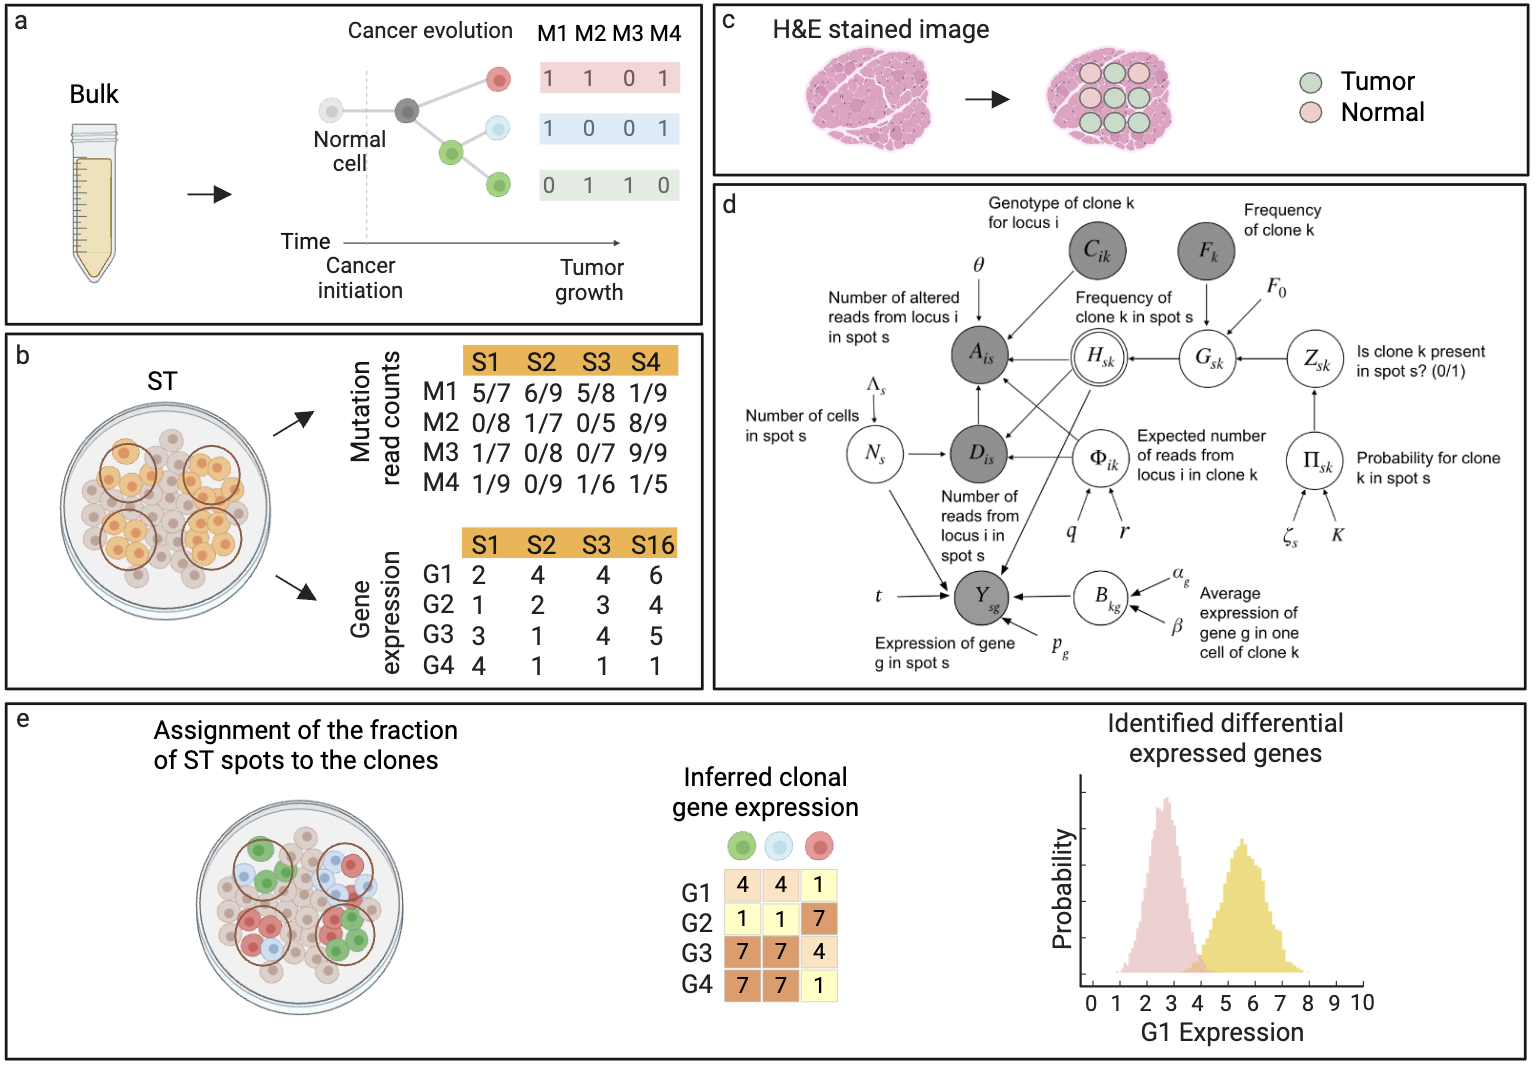
\includegraphics[scale=0.5]{figures/overview.png}
\caption{\textbf{\bf{ClonalGE framework overview.}} {\bf a-c} Data preprocessing. Tumor clones, their genotypes and frequencies are found from DNA-seq data ({\bf a}). Alternated to total readcounts at the SNV sites and gene expression measurements for genes in the cancerous spots are identified in ST data ({\bf b}). Cancerous regions are identified and initial cell counts are found from H\&E images of the tumor tissue ({\bf c}). {\bf d} ClonalGE probabilistic model\rev{; a complete list of all variables and parameters is provided in Supplementary Table~S1}. {\bf e} Outputs:  Inferred fraction of the clones in the spots, inferred clonal gene expression, and identified differentially expressed genes.}\label{fig:overview}
\end{figure*}
\begin{methods}
\section{Methods}
%\subsection*{A novel framework for inference of gene expression profiles specific for cancer clones, together with spatial mapping of the clones in tumor tissue and estimation of differential gene expression between clones}
\subsection*{ClonalGE framework overview}

We propose a novel probabilistic framework for inference of gene expression profiles of cancer clones, alongside the spatial mapping of the clones across the tissue and estimation of differential gene expression between the clones, using H\&E stained images, spatially-resolved transcriptomics, and bulk DNA-seq. This framework takes as input  pre-processed data, including: genotypes and frequencies of the inferred clones (based on bulk DNA-seq data; Fig.~\ref{fig:overview}a),  the total and alternated read counts over selected mutations (based on ST reads; Fig. \ref{fig:overview}b), the gene expression profile of the spots (based on ST reads; Fig. \ref{fig:overview}b), and regions of the tissue annotated as cancer and the number of cells in the annotated ST spots (based on H\&E images; Fig.~\ref{fig:overview}c), . 

The core of the framework is a probabilistic graphical model called ClonalGE. ClonalGE combines inference of clonal gene expression and composition of ST spots. The model is a profound extension of our previous model, Tumoroscope~\citep{shafighi2024integrative}, by incorporating additional variables for the gene expression in the spots. The assumptions behind this extension are that each clone has its specific average gene expression profile; and that the expression of the genes observed at the spots is a mixture of the gene expressions in the clones that are present in those spots. For inference, we proceed in two stages. Tumoroscope is run first to provide initialisation of all the hidden variables to ClonalGE. In the second stage, we use Metropolis Hastings within Gibbs for estimation of ClonalGE (Fig. \ref{fig:overview}d). The model returns the fraction of each annotated ST spot occupied by each clone together with the gene expression profile of each clone (Fig. \ref{fig:overview}e). Finally, we use the model-inferred distributions of gene expression for each clone to perform differential gene expression analysis between clones (Fig. \ref{fig:overview}e). The details of input data and each step of the methodology are described in the following subsections.


\subsection*{Prostate cancer sample}
We used a published prostate cancer dataset including DNA-seq, H\&E images, and ST data~\citep{berglund2018spatial}. The DNA-seq was performed on tissue layers adjacent to ST and H\&E. The data was available for twelve sections covering half of the prostate extracted by a prostatectomy on a patient with adenocarcinoma (Gs 3 + 4, pT3b, PSA 7.1). Besides, we used the DNA-seq data from the patient's blood to serve as a control for detecting the somatic mutations. 
The data generation protocol  as well as data availability were described by~\cite{berglund2018spatial}. Details of data preprocessing for ClonalGE follow the procedure of~\cite{shafighi2024integrative} and are briefly covered in the following sections.

\subsection*{Annotation of cancerous spots and counting cells in spots from H\&E images} 
%For each section, we retrieved the same spots that were identified by~\cite{shafighi2024integrative} as cancerous. 
For cancerous spot identification, the regions containing cancer cells were annotated by an expert pathologist taking advantage of the H\&E image of each section. Afterward, using a custom script in QuPath~\citep{bankhead2017qupath}, the spots inside the annotated regions were identified. These spots were located in three of the twelve original sections (named SP1, SP2 and SP3 as in~\cite{shafighi2024integrative}). 

Cells in the cancerous spots were counted using another custom script in QuPath. The script accepts input in the form of coordinates and diameters of spots to define target regions. Subsequently, QuPath's built-in algorithm is utilized to detect and enumerate nuclei. The algorithm's parameters were optimized by matching the output counts with manual cell count within randomly selected spots. 

\subsection*{Somatic mutation calling from DNA-seq data}
We called somatic point mutations  using Vardict~\citep{lai2016vardict}.  The final set of  mutations contained variants called with a p-value threshold equal to 0.1 in at least one of the DNA-seq sections (i.e., the set of mutations was the union over mutations found in individual sections). \rev{Initially, 2104 somatic mutations were called across all sections. After filtering for presence in both DNA-seq and ST data, 280 mutations remained and were used for downstream analysis.}

\subsection*{Extraction of read count data for  somatic mutations that were detected both in DNA-seq and ST data}
We selected the mutations for which at least one alternated read in at least one section was found. Calculation of the the total and alternated reads over the mutations in ST data was done by a script provided by~\cite{shafighi2024integrative}, which finds the selected DNA-seq mutations in the ST bam files and counts the corresponding mapped reads.  We next gave the alternated and total read counts in DNA-seq data as input to the method of phylogenetic tree inference. Finally, we gave the alternated and total read counts in ST data for the same mutations as input to the ClonalGE model. 

\subsection*{Estimation of the genotypes and frequencies of the  clones from DNA-seq data}
The genotypes and frequencies of the clones were obtained using a statistical method for inference of  phylogenetic trees called Canopy~\citep{jiang2016assessing}. Canopy takes the following inputs: 1) variant allele frequencies (VAF) of somatic single nucleotide alterations, obtained by Vardict~\citep{lai2016vardict} and 2) ratios of the coverage between the tumor and normal sample for somatic copy number alterations (CNAs), obtained by FalconX~\citep{chen2017allele}. We used the multi-sample feature of the Canopy  to infer the clonal evolution across the sections. Clone 1 returned by Canopy should be considered  normal  (without any somatic mutations).


\subsection*{ClonalGE}\label{s:my_model}
ClonalGE is a probabilistic graphical model for estimating the gene expression profile of the clones alongside with the fraction of the clones in the ST spots across the tumor sample. 

Let $k \in \{1, \ldots, K\}$ index the clones derived from DNA sequencing data and $i \in \{1, \ldots, I\}$ index the loci with somatic point mutations observed both in ST and DNA-sequencing data. $F_k$ indicates the frequency of occurrence of clone $k$ in the whole sample. $C_{ik}$ codes the inferred genotype, taking values between 0 and 1, and  is defined by the ratio of the number of alleles of clone $k$ carrying a mutation on locus $i$ to the total number of alleles. Both the frequencies $F_k$ and genotypes $C_{ik}$ are specifications of the clones estimated from DNA-seq data and are considered as observed variables in the model. 

Let $s \in \{1, \ldots, S\}$ index the spots in the ST data. $Z_{sk}$ is a hidden binary variable, indicating the presence of clone $k$ in spot $s$. It follows a Bernoulli distribution with success parameter   $\Pi_{sk}$, following a Beta prior distribution.
$$\mathbb{P}(Z_{sk}|\Pi_{sk}) \; \sim \; \mathrm{Bern}(\Pi_{sk}),$$
$$\mathbb{P}(\Pi_{sk}|\zeta_s,K) \; \sim \; \mathrm{Beta}\left(\frac{\zeta_s}{K},1\right).$$
The hyperparameter $\zeta_s$ influences expected number of clones in a spot, which is given by $$\frac{\zeta_s}{\zeta_s+K}.$$
%Italic will denote the density distribution function

Depending on the indicator variables $Z_{sk}$ and the observed clone genotypes and frequencies, we expect higher or lower values of unnormalized abundances of the clones in the spots. These unnormalized abundances for each spot $s$ and clone $k$ are described in the model using Gamma-distributed hidden variables $G_{sk}:$
$$\mathbb{P}(G_{sk} | F_k, F_0, Z_{sk}) \; \sim \; \mathrm{Gamma}({f(F_{k})}^{Z_{sk}}{F_{0}}^{1-Z_{sk}},1).$$
The first parameter of the Gamma distribution is calculated using a discretized value of $F_k$. The discretization is performed for technical reasons and helps avoid numerically too small values. \rev{Specifically, when clone frequencies $F_k$ are very small, the shape parameter of the Gamma distribution for $G_{sk}$ approaches zero, leading to numerically degenerate distributions where nearly all probability mass concentrates at zero. The discretization ensures a minimum effective shape parameter, preserving numerical stability while maintaining the relative ordering of clone frequencies. The discretization level of $0.05$ was chosen to balance numerical stability with the resolution of frequency differences.} The discretization function $f$ is  defined by $f(x) = \lceil \frac{x}{0.05}\rceil \cdot 100$. The hyperparameter $F_0$ is used as a pseudo-count for clones not assigned to the spot, indicated by $Z_{sk}=0$, and is set to a small number.

$H_{sk}$ is a deterministic variable that can be interpreted as a fraction of spot $s$ assigned to clone $k$. It follows a Dirichlet distribution and is calculated based on the unnormalized abundances $G_{sk}$ as $$H_{sk} = \frac{G_{sk}}{\sum_{l=1}^{K} G_{sk}}.$$
Note that $H_{sk}$'s are one of the two central sets of random variables in the model - they solve the task of identifying the proportions of the clones in the spots.

$\Phi_{ik}$ is a latent variable that is interpreted as an average read count at position $i$ per one cell of clone $k$. It follows a Gamma distribution with hyperparameters $r$ and $q$:
$$\mathbb{P}(\Phi_{ik}|r,q) \; \sim \; \mathrm{Gamma}(r,q).$$
The number of cells in spot $s$, represented by a variable $N_s$ is modeled with a Poisson distribution:
$$\mathbb{P}(N_s|\Lambda_s) \; \sim \; \mathrm{Poiss}(\Lambda_s),$$
where $\Lambda_s$ is the provided at input  cell count at spot $s$, estimated from H\&E images.

$D_{is}$ represents counts of reads over locus $i$ coming from spot $s$ and $A_{is}$ indicates how many of them are mutated (altered). $D_{is}$ and $A_{is}$ are observed variables extracted from ST reads and are given to the model and assumed to follow a Poisson distribution and a Binomial distribution respectively:
$$\mathbb{P}(D_{is}|H_{s.},\Phi_{i.},N_s) \; \sim \; \mathrm{Pois} \left(N_s\sum_{k}{H_{sk}\Phi_{ik}}\right),$$
$$\mathbb{P}(A_{is}|D_{is},\Phi_{i.},H_{s.},C_{i.}) \; \sim \; \mathrm{Binom} \left(D_{is},\frac{\sum_{k}\Phi_{ik}C_{ik}H_{sk}}{\sum_{k}\Phi_{ik}H_{sk}}\right).$$

All the above definitions concern also the previous model Tumoroscope by~\cite{shafighi2024integrative}. We now explain the model extension to account for gene expression values in the spot, allowing to estimate gene expression profiles of clones as an integral part of the model.

Let $g \in \{1, \ldots, G\}$ index the genes observed in the ST data. Our main goal is to estimate the average gene expression of gene $g$ per one cell in clone $k$, represented by a hidden random variable $B_{kg}$, which is the second central variable in the model and is assumed to follow a Gamma distribution with hyperparameters $\alpha_{g}$ and $\beta$
$$\mathbb{P}(B_{kg}|\alpha_{g},\beta) \; \sim \; \mathrm{Gamma}(\alpha_{g},\beta).$$

An observed variable $Y_{sg}$ signifies the expression of gene $g$ in spot $s$ which is the main measurement in ST data and is given to the model at input. We assume a Negative Binomial distribution over $Y_{sg}$ with expected value of $N_s\sum_{k}{H_{sk}B_{kg}}$, which is the clonal gene expression multiplied by the number of cells of each clone in spot $s$. To overcome the batch effect observed when integrating the data from different sections, we added a scaling parameter $t_j$ to the model (with $j$ indexing the sections and $t_j$  assumed to be common for all spots in  section $j$). Then the expected value for $Y_{sg}$ is $t_j \cdot N_s\sum_{k}{H_{sk}B_{kg}}$ given that spot $s$ is in section $j$. Considering $r_{sg}$ and $p_{g}$ as the parameters of the Negative Binomial distribution over $Y_{sg}$, the expected value of $Y_{sg}$ is $\mathbb{E}[Y_{sg}] = \frac{(1-p_{g})r_{sg}}{p_{g}}$ and the variance is equal to $Var(Y_{sg}) = \frac{(1-p_{g})r_{sg}}{p_{g}^2}$. Using the formula for $\mathbb{E}[Y_{sg}]$ we substitute $r_{sg}$ by
$$r_{sg} =\frac{\mathbb{E}[Y_{sg}]p_{g}}{1-p_{g}},$$
which results in a useful reparametrization:
\begin{equation} \label{eq:NB}
Y_{sg} \sim \mathrm{NB}\left(\frac{\mathbb{E}[Y_{sg}]p_{g}}{1-p_{g}}, p_{g}\right).
\end{equation}
\rev{This reparameterization is advantageous because it expresses the distribution directly in terms of the expected gene expression $\mathbb{E}[Y_{sg}]$, which can be linked to the biologically meaningful clone-weighted expression contributions $N_s\sum_{k}{H_{sk}B_{kg}}$, while retaining the overdispersion properties of the Negative Binomial distribution appropriate for count data.}
Using this parametrization, we can rewrite the distribution of $Y_{sg}$:
$$\mathbb{P}(Y_{sg}|t_j, B_{.g},p_g,H_{s.},N_s) \; \sim \; \mathrm{NB} \left(t_j N_s\sum_{k}{H_{sk}B_{kg}}\frac{p_g}{1-p_g},p_g\right),$$
where spot $s$ is in section $j$.

\subsection*{Metropolis-Hasting inside Gibbs sampling}
For estimating the posterior distribution of the hidden variables in our probabilistic model, we iteratively generate samples from each hidden variable's conditional distribution, given the remaining variables. We use a Metropolis-Hasting step inside the Gibbs sampler in case a closed-form distribution for sampling a random variable does not exist. 

The sampling procedure for variables $\Phi_{ik}$, $Z_{sk}$ and $\Pi_{sk}$ remain the same as is described in \cite{shafighi2024integrative}. Here we describe the sampling procedure for the remaining part of the model. 

We use Metropolis-Hastings inside Gibbs sampler for variables  $G_{sk}$, $N_s$ and $B_{kg}$ since there exists no closed form of their full conditional distributions. We choose a Truncated Normal distribution for the proposal distribution due to the non-negativity of these variables. 
%$x_c$ represents the mean value and $\sigma_{G}$ and $\sigma_{N}$ represent the variances of the proposal distribution corresponding to each variable. 
The proximity of the new sample from the current one, which is interpreted as the step size, is determined by the variance of the proposal distribution. During the sampling steps, we learn the optimal variance value for each variable as described by~\cite{shafighi2024integrative}. 


Conditional distribution for $G_{sk}$:
\begin{multline*}
\mathbb{P}(G_{sk}|F_k,F_0,Z_{sk}, A_{is}, D_{is})\\
\propto \mathbb{P}(G_{sk}|F_k,F_0,Z_{sk})\prod_i \mathbb{P}(D_{is}|\Phi_{i.},H_{s.},N_s) \\ \times \prod_i\mathbb{P}(A_{is}|D_{is},\Phi_{i.},H_{s.},C_{i.})
\\ \times \prod_g \mathbb{P}(Y_{sg}|t, B_{.g},p_g,H_{s.},N_s)\\
= Gamma({f(F_{k})}^{Z_{sk}}F_{0}^{1-Z_{sk}},1) \prod_i Pois (N_s\sum_{k}{H_{sk}\Phi_{ik}}) \\ \times \prod_i Binom (D_{is},\frac{\sum_{k}\Phi_{ik}C_{ik}H_{sk}}{\sum_{k}\Phi_{ik}H_{sk}}) \\ \times \prod_g NB(t N_s\sum_{k}{H_{sk}B_{kg}}\frac{p_g}{1-p_g},p_g),
\end{multline*}
where with italic names we write the density functions of the respective probability distributions.\\
Conditional distribution for $N_{s}$:
\begin{multline*}
\mathbb{P}(N_{s}|\Lambda_s, D_{is}, Y_{sg})
\propto \mathbb{P}(N_{s}|\Lambda_s) \\ \times \prod_i\mathbb{P}(D_{is}|\Phi_{i.},H_{s.},N_s) 
 \prod_g \mathbb{P}(Y_{sg}|t, B_{.g},p_g,H_{s.},N_s)\\
=Pois(\Lambda_s)\prod_i Pois (N_s\sum_{k}{H_{sk}\Phi_{ik}})\\ \times \prod_g NB(t N_s\sum_{k}{H_{sk}B_{kg}}\frac{p_g}{1-p_g},p_g).
\end{multline*}
Conditional distribution for $B_{kg}$:
\begin{multline*}
\mathbb{P}(B_{kg}|\alpha_g, \beta, Y_{sg})
\propto \mathbb{P}(B_{kg}|\alpha_g, \beta) \prod_s \mathbb{P}(Y_{sg}|t, B_{.g},p_g,H_{s.},N_s)\\
= Gamma(\alpha_{g},\beta) \prod_s NB(t N_s \sum_{k}{H_{sk}B_{kg}}\frac{p_g}{1-p_g},p_g).
\end{multline*}


\subsection*{Hyper-parameter estimation and initialization of random variable values prior to MCMC}
%We firstly run the Tumoroscope model and use the inferred values of the hidden variables $H$ and $N$ to initialize the respective hidden variables $H$ and $N$ of ClonalGE. We further use the regression model proposed in ~\cite{shafighi2024integrative} to initialize the $B$ matrix.

We estimate the hyper-parameters of the model based on the real data. First, the value of  $\Lambda_s$ is set to the estimated number of cells in spot $s$, calculated based on the H\&E images. 
Second, having a Negative Binomial distribution over $Y_{sg}$ with the success probability $p_g$, we have $$p_g  = \frac{\mathbb{E}[Y_{sg}]}{Var(Y_{sg})}.$$
Thus, we approximate $p_g$ by estimating $\mathbb{E}[Y_{sg}]$ and ${Var(Y_{sg})}$ using arithmetic mean and the variance of the given gene expression data for gene $g$ over the spots. 

For estimating the gene expression scaling factor, $t_j$, we calculate the mean value of $Y_{sg}$ for spots $s$ that are present in section $j$. Let $m_{1},\ldots, m_{J}$ be the average gene expression for spots in the $J$ analyzed sections and let $m = \frac{1}{J}(m_{1} + \ldots + m_{J})$. Then for section $j$ the estimated scaling factor is $\hat{t}_{j} = \frac{m_{j}}{m}$.

For estimating the hyperparameters $\alpha_g$ and $\beta$ of the Gamma distribution of the $B_{kg}$ variables %$$\mathbb{P}(B_{kg}|\alpha_{g},\beta) \; \sim \; Gamma(\alpha_{g},\beta),$$ 
we use the formulas for expected value, $\mathbb{E}[B_{kg}] = \alpha_g\beta$, and the variance, $Var(B_{kg}) = \alpha_g\beta^2$ of the Gamma distribution. Therefore, one could obtain  $\beta$ by dividing the two values.$$\beta = \frac{Var(B_{kg})}{\mathbb{E}[B_{kg}]}.$$
Since we do not have $B$ values as they are latent variables, we approximate them by the average expression of the gene per cell over clones: 
$$B_{kg} \approx \frac{\sum_{k=1}^{K} B_{kg}}{K} \approx \frac{1}{S\cdot J} \sum_j \sum_{s \textrm{ in section } j} \left(\frac{Y_{sg}}{t_j N_s}\right).$$
Therefore, we estimate $\mathbb{E}[B_{kg}]$ and $Var(B_{kg})$ by calculating the mean and variance of these average values across genes. By considering the average over clones, we are underestimating the variance and accordingly the values of $\beta$. Therefore, we multiply the estimated variance by a correction parameter $\omega_{B}$. The value of $\omega_{B}$ was estimated based on simulations and fixed to $\omega_{B}=2$.

%we approximate them using the equation $\mathbb{E}[Y_{sg}] = tN_s\sum_{k}{H_{sk}B_{kg}}$ and estimate $B_{.g}$ with $$E(B_{.g})\approx \frac{\mathbb{E}[Y_{sg}]}{tN_s} \approx \frac{1}{S} \sum_s (\frac{Y_{sg}}{tN_s}) \approx \frac{1}{S} \sum_s (\frac{Y_{sg}}{\hat{t}\Lambda_s}) = \hat{B}_g$$
%and then $$\hat{\beta} \approx \frac{var(\hat{B}_g)}{mean(\hat{B}_g)}.$$ Since we are underestimating $\beta$ by this estimation, we multiply the result by a constant $\omega_{B}$. $$\beta \approx \omega_B\frac{var(\hat{B}_g)}{mean(\hat{B}_g)}.$$
%Analysis conducted on simulated data has shown that $\hat{\beta} = 2\frac{var(\hat{B}_g)}{mean(\hat{B}_g)}$ gives good estimates.\\
Next, based on the expected value of the Gamma distribution over $B_{kg}$, $\mathbb{E}[B_{kg}] = \alpha_g\beta$, 
we approximate $\alpha_g$ using the estimated $\hat{\beta}$ and the already calculated average expression of the genes over the clones. 
%and the already estimated $\hat{\beta}$, $$\mathbb{E}[B_{kg}] = \alpha_g\beta \Rightarrow \hat{\alpha}_g = \frac{\hat{B}_g}{\hat{\beta}}$$

We estimate the hyper-parameters of Gamma distribution over $\Phi$, $r$ and $q$, similarly to the $\alpha_g$ and $\beta$, using the approximation of the expected value and variance of $\Phi$. 
$$\hat{E}(\Phi) = \frac{\sum_{i}\sum_{s}\frac{D_{is}}{N_s}}{I\times S} $$
$$\hat{Var}(\Phi) =\frac{\sum_{i}\sum_{s}(\frac{D_{is}}{N_s}-E(\Phi))}{I\times S}.$$
Then, we estimate the hyper-parameters with $$\hat{r} = \omega_{\phi}\frac{\hat{Var}(\Phi)}{\hat{E}(\Phi)} \text{\quad and\quad} \hat{q} = \frac{\hat{E}(\Phi)}{\hat{r}}.$$
Here, we use a constant, $\omega_{\phi}$, for compensation of the underestimation of the $r$. This correction constant was again estimated based on simulations and fixed to $\omega_{\phi}=2$.


%We firstly run the Tumoroscope model and use the inferred values of the hidden variables $H$ and $N$ to initialize the respective hidden variables $H$ and $N$ of ClonalGE. We further use the regression model proposed in ~\cite{shafighi2024integrative} to initialize the $B$ matrix.
 To find initial values of hidden variables prior to MCMC, we first run Tumoroscope for at least 7000 iterations stopping after reaching the Geweke's convergence criterion~\citep{geweke1991evaluating}, with the upper bound of 15000 iterations. Afterward, we use the inferred variables to initialize the corresponding hidden variables in ClonalGE. We further use the regression model proposed in ~\cite{shafighi2024integrative} to initialize the $B$ matrix.
 
\subsection*{Examining convergence }
We examine the convergence of the MCMC for ClonalGE by using  Geweke's convergence diagnostic on the $H$ variable matrix. We consider different sizes of the burn-in period and examine them by calculating the percentage of the convergence after each batch (we use batches of 1000 iterations). We finish the sampling process if at least $99.5\%$ of the iterations have already converged and the sampling has reached a selected minimal number of iterations.

\subsection*{Inferring the variables based on the samples}
For the real data, we compute final values of the inferred variables using multiple chains. Specifically, we run the model 10 times, each time with 10 chains. Then, from each run we select the chain with the highest likelihood, and all chains that obtained similar results. We consider two chains similar if the Pearson correlation between the inferred $H_{sk}$ values is higher than $0.9$. If the chain with the highest likelihood does not have any other similar chains, we omit it. Afterward, we take an average out of all the chains that are similar to the one with the highest likelihood out of the remaining chains.

\subsection*{Differential gene expression analysis between clones}
\rev{We obtain posterior pseudo-samples of the inferred gene expression per clone $k$ and gene $g$ using batch means computed from the post-convergence MCMC iterations. Specifically, the post-burn-in iterations are divided into batches of $b$ MCMC steps; within each batch the $b/t$ thinned $B_{kg}$ values (thinning factor $t$) are averaged to form one batch-mean pseudo-sample vector per chain. These batch-mean pseudo-samples are pooled across all consensus-selected chains and runs, yielding a set of $S$ posterior pseudo-samples in total. For each gene $g$ and each pair of clones $(k_1, k_2)$, we then estimate the posterior probability of differential expression as:
$$P(B_{k_1,g} > B_{k_2,g} \mid \text{Data}) \approx \frac{S_{>}}{S},$$
where $S_{>}$ is the number of pseudo-samples in which $B_{k_1,g} > B_{k_2,g}$. A gene is considered differentially expressed between two clones when this posterior probability exceeds $0.95$ (or falls below $0.05$). This Bayesian approach is coherent with the probabilistic framework of ClonalGE and provides a directly interpretable measure of evidence for clone-specific differential expression. We compute this statistic} for each pair of clones, excluding the normal clone 1, and each gene from a given set of $n$ genes.
% Updated: batch-mean pseudo-samples replace the earlier "every 1000-th sample" description

\subsection*{Computing the expected gene expression values across spots based on the inferred clonal gene expression profiles}
%We use a regression model for estimating the average clonal gene expression by a python function $scipy.optimize.lsq\_linear$ as it proposed in Tumoroscope~\cite{shafighi2024integrative}. 
Having the inferred clonal expression $B_{kg}$, we compute the expected gene expression profile across spots in the tissue section $j$ as:
$$\hat{Y}_{sg}~=~\sum_{k}t_jN_s{H_{sk}B_{kg}} = t_jN_s\sum_{k}{H_{sk}B_{kg}}.$$ 
\begin{figure*}[!t]%figure1
\centering
%\includegraphics{figures/sim}
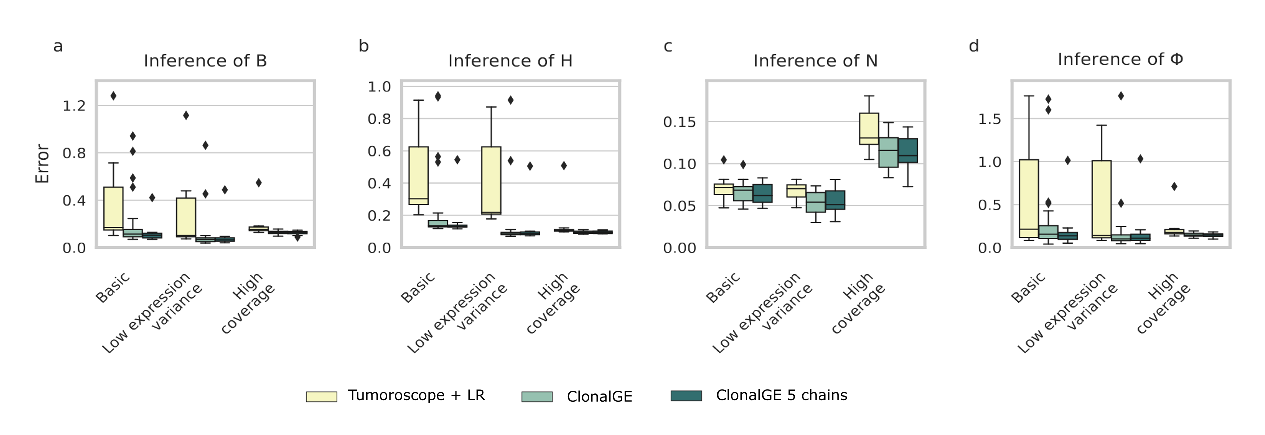
\includegraphics[width=0.9\textwidth]{figures/simulations.eps}
\caption{{\bf Performance of ClonalGE on simulated data.} \textbf{a} \rev{Relative Mean Absolute Error (rMAE, defined as the Mean Absolute Error divided by the mean of the true values; y-axis)} of inferred clonal gene expression profile in different simulation setups (x-axis) for different methods (colors). {\bf{b}} The same as in ({\bf a}), but for the inferred fraction of the clones in the spots. {\bf{c}} The same as in ({\bf a}), but for the corrected number of cells in the spots.
{\bf{d}} The same as in ({\bf a}), but for the inferred number of total reads per cell in each clone.
}\label{fig:perfsim}
\end{figure*}
\subsection*{Generating simulated data}
The data were simulated from the ClonalGE model. To this end, we first fixed the hyperparameters, and next sampled each variable conditional on its parents' values, following the order of the variables in the graphical model~(Fig.\ref{fig:overview}d). 

Specifically, we generated data in three setups. First, the {\it basic} setup, with $K=5$ clones randomly mixed in $S=300$ spots, total number of  mutations  set to $I=200$ and the number of analyzed genes $G=50$. 
We fixed the hyperparameter $\Lambda_s$ so that the expected value for the number of cells was 45,  and the hyperparameter $\zeta_s$ so that the expected number of clones in each spot $s$ was 2.5. 
We fixed the hyperparameters $r$ and $q$ to $0.005$ and $1$ so that the sum of simulated read counts per each spot was in the (36, 44) interval
, and the expected value of gene expression variance for the genes across the spots was 1715, reflecting the levels observed in real data. 

Next, to test the influence of  the different gene expression levels and the coverage per mutation, we designed two additional setups ({\it low expression variance} and {\it high coverage}). These setups were obtained as the {\it basic} setup, but lowering the expected value of the expression variance and increasing the average number of reads, respectively (see Table~\ref{tab:sim}). For each setup, we repeated the simulation 20 times, obtaining a total of 60 simulated datasets.

\begin{table}[!h]
{\small{
{\begin{tabular}{|l|l|l|l|}
\hline 
 \multicolumn{1}{|p{2.5cm}|}{\centering setup \\ property }
& \multicolumn{1}{|p{1cm}|}{\centering {\textit{basic}} \\  }
& \multicolumn{1}{|p{1.8cm}|}{\centering {\textit{low expression \\ variance}} }
& \multicolumn{1}{|p{1.2cm}|}{\centering {\textit{high \\ coverage }}}\\\hline
  \multicolumn{1}{|p{2.5cm}|}{\centering interval of the \\ average read counts  }
& \multicolumn{1}{|p{1cm}|}{\centering $(36, 44)$   }
& \multicolumn{1}{|p{1.8cm}|}{\centering $(36, 44)$  }
& \multicolumn{1}{|p{1.2cm}|}{\centering $(180, 221)$   }\\\hline
  \multicolumn{1}{|p{2.5cm}|}{\centering expected value of   \\ expression variance}
& \multicolumn{1}{|p{1cm}|}{\centering 1715 }
& \multicolumn{1}{|p{1.8cm}|}{\centering 315 }
& \multicolumn{1}{|p{1.2cm}|}{\centering 1715 }\\\hline
\end{tabular}}{\caption{Parameters for generating three different simulation setups.}\label{tab:sim}}
}}
\end{table}
\end{methods}



\section{Results}
\subsection*{ClonalGE outperforms predecessor model on simulated data}
We first assessed the performance of ClonalGE on simulated data, where the ground truth was known, for  three different simulation setups: {\textit{basic}}, {\textit{low expression  variance}}, and {\textit{high  coverage }} (see Methods).

 For inference, we first ran the sampling process of ClonalGE for at least 10000 iterations, saving every 5th sample and stopping after reaching convergence with an upper bound of 30000 iterations. The initial parameters were set using a pre-run of Tumoroscope (see Methods). We discarded the burn-in samples and used the remaining for inference of the latent variables. We used known values of the hyper-parameters, except for $r$ and $q$, which were estimated (see Methods). We also evaluated another running procedure of ClonalGE that aimed at decreasing the chances of getting stuck in local optima. To this end, we ran five MCMC chains for ClonalGE and selected the chain with the highest likelihood. This procedure is referred to as ClonalGE 5 chains.

For comparison, we ran Tumoroscope with its parameter estimation procedure for the same lower and upper bound numbers of iterations as ClonalGE. 
To estimate gene expression per clone after running Tumoroscope, 
similarly to~\cite{shafighi2024integrative}, we used linear regression (LR) with weights fixed to the  fractions of clones in spots inferred by Tumoroscope. Hence, this entire procedure is referred to as Tumorocope + LR.   

Overall, both ClonalGE and ClonalGE 5 chains obtained significantly better results compared to Tumoroscope + LR in all simulation setups (Fig.~\ref{fig:perfsim}). In particular, ClonalGE obtained much more accurate estimates of gene expression values in clones (Fig.~\ref{fig:perfsim}a). This result confirms that the joint modeling of the gene expression values
with the mutation read counts as performed in ClonalGE gives increased statistical strength and yields higher performance than the double step procedure employed by combining Tumoroscope with linear regression. This advantage may also come from the appropriate model of the Negative Binomial distribution for the expression data per gene and spot employed by ClonalGE, in contrast to linear regression.

\rev{To disentangle the contribution of the Negative Binomial distribution from the benefit of joint inference, we additionally compared ClonalGE against Tumoroscope followed by Negative Binomial regression (Tumoroscope + NB), where gene expression per clone is estimated using a Negative Binomial generalized linear model with weights fixed to the Tumoroscope-inferred clone fractions. While Tumoroscope + NB improves upon Tumoroscope + LR for gene expression estimation (Fig.~\ref{fig:perfsim}a), ClonalGE still achieves superior accuracy across all variables. This confirms that the integrated probabilistic inference framework provides benefits beyond adopting a more appropriate count distribution in a post-processing step (Fig.~\ref{fig:perfsim}).}

Interestingly, ClonalGE also outperforms Tumoroscope in the functionality that is shared between these two models: inference of the fraction of clones in spots (Fig.~\ref{fig:perfsim}b), numbers of cells in spots (Fig.~\ref{fig:perfsim}c), and read coverages per mutation per cell (Fig.~\ref{fig:perfsim}d). 
%by keeping the inferred number of reads close to the true, simulated values for {\it basic} and {\it low expression variance} setups. 
%These results signify the higher sensitivity of  Tumoroscope to the number of reads than ClonalGE. 
This is likely due to the fact that ClonalGE, in contrast to Tumoroscope, benefits from the additional signal in gene expression measurements across spots. 
The most significant improvement over Tumoroscope is visible for the {\it basic} and {\it low expression variance} setups, both characterized by low coverage. 
%In both these setups, the coverage is low. 
These demanding setups illustrate that Tumoroscope is more sensitive to coverage than ClonalGE.

%The higher number of reads improved the accuracy of the inferred fraction of the clones in the spots(median relative MAE from 0.302, 0.135, 0.131 to 0.106, 0.094, 0.093, for Tumoroscope, ClonalGE and ClonalGE 5 chains respectively; Supplementary table 1). On the other hand, it impaired the accuracy of the estimated number of cells in the spots (median relative MAE from 0.071, 0.068, 0.062 to 0.130, 0.115, 0.109, for Tumoroscope, ClonalGE, and ClonalGE 5 chains respectively; Supplementary table 1). 

%The lower gene expression variance  improved the clonal gene expression estimation (median relative MAE from 0.168, 0.113, 0.104 to 0.101, 0.067, 0.064, for Tumoroscope, ClonalGE, and ClonalGE 5 chains respectively; Supplementary table 1).  

As expected, ClonalGE with five chains achieved more robust results with lower outliers compared to both ClonalGE and Tumoroscope + LR. The mean and median of the error in all the setups and variables decreased or stayed equal when we used five chains instead of one. These results emphasize the importance of running more chains to decrease the probability of the model getting trapped in the local minimum.

%[I should mention phi in the results]
\begin{figure*}[t!]%figure1
\centering
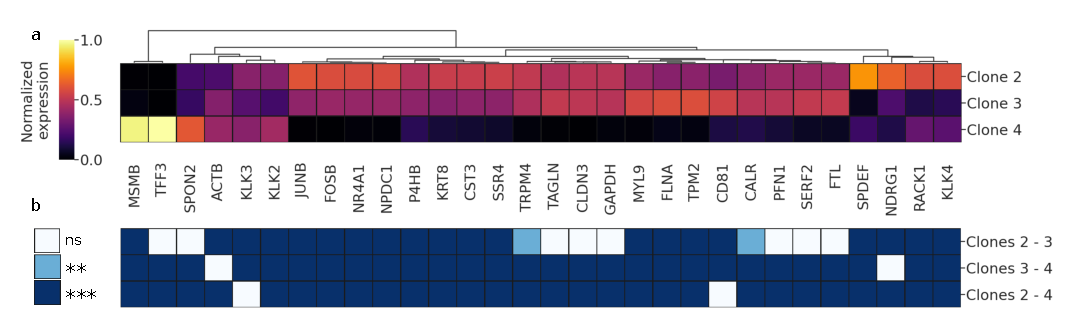
\includegraphics[width=0.9\textwidth]{figures/B.eps}
\caption{{\bf Genes are expressed differently in various cancer clones.} {\bf{a}} \rev{Normalized} expression of the 30 genes that were inferred by ClonalGE as the most active in at least one clone, clustered in rows and columns, for prostate cancer tissues. \rev{For each gene, the inferred clone-specific expression $B_{kg}$ is min-max scaled to $[0, 1]$ across clones, where $0$ and $1$ correspond to the minimum and maximum inferred expression of each gene across the clones, respectively.} {\bf{b}} \rev{Posterior probability of differential gene expression between pairs of clones, computed as $P(B_{k_1,g} > B_{k_2,g} \mid \text{Data})$ from the MCMC samples (see Methods).} }\label{fig:B_selected}
\end{figure*}

\begin{figure}[!t]
\centering
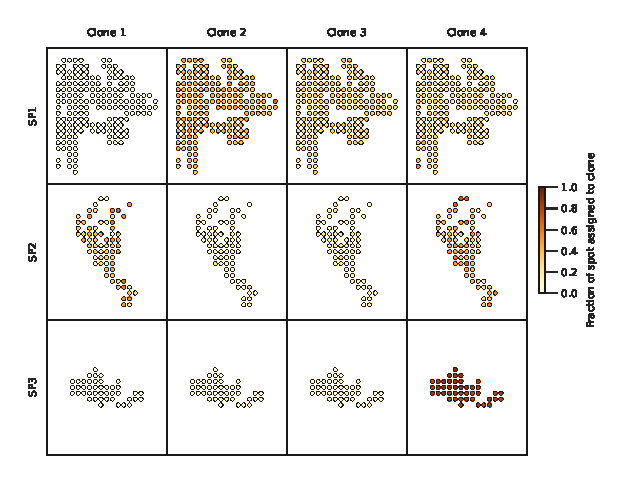
\includegraphics[width=\columnwidth]{figures/real_H.eps}
\caption{ The proportion of the spots assigned by ClonalGE to each clone (columns) for each section (rows) of the prostate sample.}\label{prostate}
\end{figure}
% This section should go first$
\subsection*{ClonalGE reconstructs the gene expression profile of the clones on prostate cancer data}
To showcase the performance of ClonalGE on real data, we applied it to prostate cancer dataset generated by~\cite{berglund2018spatial}. To this end, we selected 3 sections: SP1, SP2, and SP3 out of 12 sections, based 
on a pathologist's annotation of cancer regions. These sections were sampled from one patient, for which deep DNA-seq and ST data (custom arrays) of neighboring layers were generated~\citep{berglund2018spatial}. From these sections, only the spots overlapping with cancer regions were selected, namely 198, 70, and 43 spots from sections SP1, SP2, and SP3 respectively, out of 968-1001 spots per section. Furthermore, we excluded 17 spots in section SP3 that lacked gene expression data. In the remaining 294 spots, the sequenced transcripts were mapped to 12873 different genes. We selected the data for the 1000 most variable genes to 1) limit the computation time and 2) concentrate on the genes that carry the most information for more accurate inference. \rev{We note that this pre-selection strategy, while computationally efficient and focused on informative signals, may miss genes with subtle but consistent clone-specific expression patterns that do not exhibit high overall variance across spots.} We used the mutations present in both DNA-seq and ST data together with the  evolutionary tree reconstructed from DNA-seq data (Methods; \cite{shafighi2024integrative}). The tree included a normal clone without somatic mutations and three other clones. Finally, we applied ClonalGE to deconvolute the transcriptomic signal from the 294 cancerous spots in the ST data in order to achieve the proportions of the underlying clones and the expression profile of the clones.

For running the model on the prostate cancer dataset, we used the same procedure and number of iterations as described for the simulated data. We repeated the sampling and inference 20 times, with different random seeds, and selected only the run with the highest likelihood. For the real data, the true values of the hyperparameters are unknown and estimated (see Methods).

Finally, after inferring the gene expression profile of the clones, we ranked the genes based on the maximum expression variance of the genes across the clones in the inferred clone-specific gene expression profiles. Afterwards, we selected top 30 genes and plotted the normalized expression across the clones (Fig. \ref{fig:B_selected}a). According to the Human Protein Atlas ~\citep{ponten2008human}, top 9 out of 30 ranked genes ({\it MSMB}, {\it SPON2}, {\it KLK3}, {\it KLK2}, {\it NPDC1}, {\it TRPM4}, {\it TAGLN}, {\it CLDN3}, {\it SPDEF}, {\it KLK4}) were found to have elevated expression in all prostate cancer tissues and can be referred to as "prostate enhanced genes". %We found that 18 out of 30 genes, and 5 out of 9 prostate enhanced genes are found by \cite{shafighi2024integrative} as well.
Among these prostate enhanced genes, there are 4 genes ({\it NPDC1}, {\it TRPM4}, {\it CLDN3}, {\it SPDEF}) that were not observed in the top ranked genes (with the highest inferred expression) found previously  for the same dataset by Tumoroscope.

\rev{Several of the top clone-specific genes have well-established roles in prostate cancer biology. {\it KLK3}, {\it KLK2}, and {\it KLK4} belong to the kallikrein family, which is central to prostate cancer diagnostics (PSA is encoded by {\it KLK3}) and has been implicated in tumor progression through androgen receptor signaling. Their differential expression across clones suggests clonal heterogeneity in androgen receptor activity. {\it MSMB}, encoding a prostate secretory protein, has been identified as a tumor suppressor in prostate cancer, and its variable expression across clones may reflect different stages of malignant progression. {\it CLDN3} (Claudin-3) is involved in tight junction formation and has been implicated in epithelial-to-mesenchymal transition in prostate cancer. To further characterize clone-specific gene sets, we performed Gene Set Enrichment Analysis (GSEA) using gene rankings based on the posterior probabilities $P(B_{k,g} > B_{\text{other},g} \mid \text{Data})$ for each clone (Supplementary Figure~\ref{fig:gsea}).}

\subsection*{MCMC samples from ClonalGE enable differential gene expression analysis between clones}
\rev{We computed the posterior probability of differential expression $P(B_{k_1,g} > B_{k_2,g} \mid \text{Data})$ for each pair of clones directly from the MCMC samples} (Methods; Fig. \ref{fig:B_selected}b).
The results indicate that the majority of the top-ranked genes exhibited \rev{high posterior probability of differential expression} across the clones. Notably, the greatest degree of similarity in gene expression was observed for clones 2 and 3, where \rev{several} genes \rev{showed posterior probabilities close to $0.5$, indicating no clear differential expression}. This similarity is also reflected in normalized gene expression profiles of clones 2 and 3 (Fig. \ref{fig:B_selected}a).

Importantly, this pair of clones (2 and 3) was found to be localized in the same area across all three sections, suggesting a  correlation between spatial localization and gene expression similarity (Fig. \ref{prostate}). Interestingly, the distribution of the clones across the analyzed tissue sections inferred by ClonalGE is different than the one inferred by Tumoroscope (compare Fig. 5 in \cite{shafighi2024integrative}), which can be attributed to the adoption of the extra information of gene expression in the inference by ClonalGE. Still, both analyses indicated similarity of clones 2 and 3 on the level of inferred gene expression and on the level of their spatial proximity in the tissue. 

%\subsection*{ClonalGE assigned the ST spots to the inferred clones in the prostate cancer dataset}
% Ewa: I moved this up
%To showcase the performance of ClonalGE on real data, we applied it to prostate cancer dataset generated by~\cite{berglund2018spatial}. To this end, we selected 3 sections: SP1, SP2, and SP3 out of 12 sections, based on a pathologist's annotation of cancer regions. %These sections were sampled from one patient, for which deep DNA-seq and ST data (custom arrays) of neighboring layers were generated~\cite{berglund2018spatial}. From these sections, only the spots overlapping with cancer regions were selected, namely 198, 70, and 43 spots from sections SP1, SP2, and SP3 respectively, out of 968-1001 spots per section. Furthermore, we excluded 17 spots in section SP3 that lacked gene expression data. In the remaining 294 spots, the sequenced transcripts were mapped to 12873 different genes. We selected the data for the 1000 most variable genes to 1) limit the computation time and 2) concentrate on the genes that carry the most information for more accurate inference. We used the mutations present in both bulk DNA-seq and ST data together with the  evolutionary tree reconstructed from DNA-seq data by~\citep{shafighi2024integrative}. The tree included a normal clone without somatic mutations and three other clones. Finally, we applied ClonalGE to deconvolute the transcriptomic signal from 294 spots in the ST data in order to achieve the proportions of the underlying clones and the expression profile of the clones.

%For running each model on the prostate cancer dataset, we used the same procedure and number of iterations described for the simulated data. We repeated the sampling and inference 20 times, with different random seeds, and selected only the best run. For the real data, the true values of the hyperparameters are unknown, so we estimated the hyperparameters (see Methods). 
% let's have it in one column

%The inferred clonal fractions by ClonalGE (Fig. \ref{prostate}) shows that SP1 is predominantly occupied by clone 2 with a mixture of clones 3 and 4, while SP2 contain clone 4 along with the normal cells. Besides, SP3 is predominantly occupied by clone 4. These results indicate that there exists some differences in the tumor allocation of Tumoroscope and ClonalGE~\citep{shafighi2024integrative}. The Tumoroscope results show that SP1 is occupied by the mixture of clones 4 and 1 in the right-hand sub-area and clones 2, 3 and 4 in the left-hand sub-area but in our results there exist not substantial difference between the right and left hand sub-areas. Besides, in the Tumoroscope results, SP2 and SP3 alongside to the clone 4 which is recognized by ClonalGE as well, contain a mixture of clones 2 and 3. The main reason for these differences is based upon the adoption of the extra information of gene expression in the inference.

\begin{figure*}[!t]%figure1
\centering
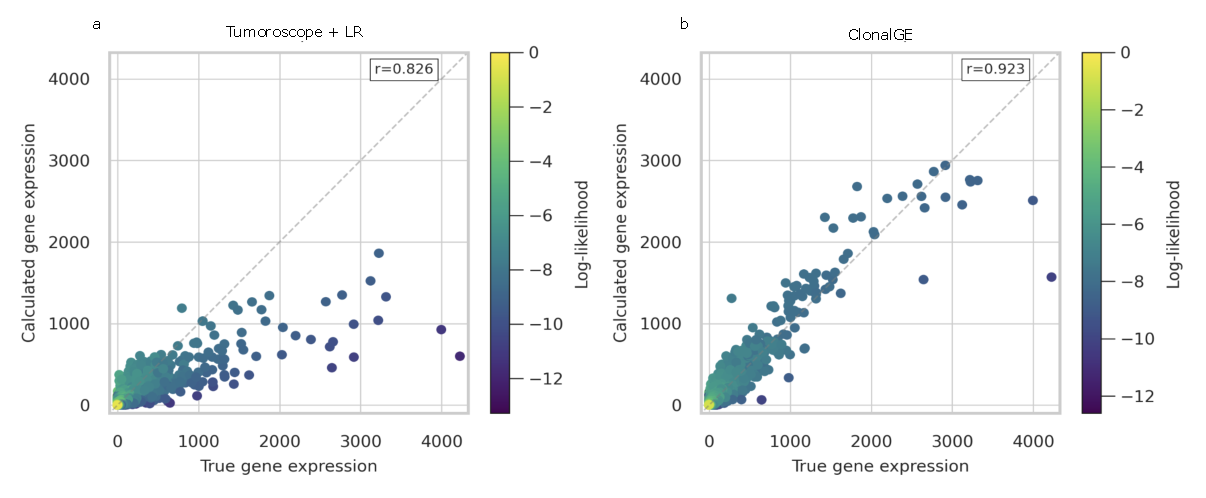
\includegraphics[width = 0.6\textwidth]{figures/Y_validation_edited.eps}
\caption{Comparison of the calculated (y-axis) and the true value (x-axis) of gene expression in the spots for  Tumoroscope followed by linear regression  (Tumoroscope + LR; {\bf{a}})  and ClonalGE ({\bf{b}}). The spots are colored based on the log-likelihood of the corresponding model.}\label{comparison}
\end{figure*}

\subsection*{ClonalGE reconstructs the gene expression profile of the tissue more accurately than Tumoroscope}

Finally, we evaluated the accuracy of the 
 gene expression reconstruction using ClonalGE. To this end, we compared the true gene expression values of the spots measured in the prostate tissue with the values expected for the same genes at the same spots based on the model estimation of clone-specific gene expression profiles (the real $\hat{Y}_{sg}$ values with the $\hat{Y}_{sg}$ values, see Methods for their calculation). For an accurate model, the real values should perfectly agree with the ones expected from the model.

For a comparison, we applied the entire procedure of Tumoroscope + LR on the same data, with the same number of iterations as for ClonalGE, and also obtained the expected gene expression values at the spots
%for Tumorscope + LR 
to compare them to the real ones. 

%Having the inferred clonal expression, the number of cells in the spots, and the fraction of the clones, we calculated the expression profile for each spot for both Tumoroscope and ClonalGE (see methods). We compared the calculated values from inferred variables with the true measured values in the ST dataset (Fig. \ref{comparison}a,b). 
We observed a much better agreement between the true gene expression values across spots and the expected values for ClonalGE than for Tumoroscope + LR  (Pearson correlation $r=0.923$ and $r=0.826$ for ClonalGE and Tumoroscope+LR respectively; see Fig. \ref{comparison}a,b). Both methods show high agreement for small expression values. However, in contrast to ClonalGE, Tumoroscope + LR tends to underestimate gene expression (Fig. \ref{comparison}a). Interestingly, the worst agreement is obtained for such genes which also have the lowest likelihood. This may be due to the fact that Tumoroscope + LR does not account for the Negative Binomial distribution of gene expression data across spots. With only a few exceptions, expected gene expression values based on ClonalGE estimates correctly recover the true measured values, even for large expression (Fig. \ref{comparison}b).

\rev{We note that this comparison evaluates the relative quality of model fit, as both methods use the observed gene expression $Y_{sg}$ during inference. Nevertheless, the comparison remains meaningful: both methods are fitted to the same data, yet achieve different levels of agreement, reflecting differences in how well each model captures the structure of spatial gene expression patterns. An ideal external validation would involve comparison against matched single-cell RNA sequencing data providing independent clone-specific expression profiles. While such orthogonal data are not available for this sample, the superior fit achieved by ClonalGE demonstrates that the integrated probabilistic framework models the spatial gene expression signal more accurately than the two-step approach.}


% ------ FIGURE -----------------------------------------------
\begin{figure}[H]
  \centering
  \includegraphics[width=\linewidth]{figures/stdeconvolve_comparison_figure.pdf}
  \caption{%
    \textbf{ClonalGE recovers clonal composition and clone-specific gene
    expression more accurately than the reference-free baseline STdeconvolve
    across all simulation settings.}
    %
    Boxplots show the Mean Absolute Error (MAE) over 20 independent simulation
    replicates for clone proportion estimation ($H$, left) and normalised
    clone-specific gene expression ($B$, right) under three simulation
    configurations: Normal, Low Variance, and High Coverage.
    %
    Fold-improvements of ClonalGE over STdeconvolve are annotated above each
    configuration group.
    %
    Lower values indicate better recovery of the ground truth.
  }
  \label{fig:stdeconvolve_comparison}
\end{figure}

% ------ TABLE ------------------------------------------------

%Comparison of clone recovery accuracy between ClonalGE and STdeconvolve on simulated data (20 replicates per configuration). Values are mean \(\pm\) standard deviation of the Mean Absolute Error (MAE) across replicates.
    %\(H\) MAE measures clone proportion recovery (lower is better);
    %\(B\) MAE measures normalised clone-specific gene expression recovery
    %(lower is better; both methods' \(B\) matrices are row-normalised to enable scale-free comparison). Fold-improvement indicates how many times lower the ClonalGE error is relative to STdeconvolve.


\begin{table}[H]
  \centering
  \caption{%
    Clone proportion recovery (\(H\) MAE; lower is better).
    Values are mean \(\pm\) standard deviation across 20 replicates.
    Fold-improvement shows how many times lower ClonalGE error is relative to STdeconvolve.
  }
  \label{tab:h_mae_comparison}
  \small
  \begin{tabular}{l c c c}
    \toprule
    Configuration
      & {ClonalGE}
      & {STdeconvolve}
      & {Fold\(\uparrow\)} \\
    \midrule
    Normal
      & \(0.0301 \pm 0.0107\)
      & \(0.0682 \pm 0.0187\)
      & \(2.3\times\) \\
    Low Variance
      & \(0.0174 \pm 0.0021\)
      & \(0.0463 \pm 0.0165\)
      & \(2.7\times\) \\
    High Coverage
      & \(0.0191 \pm 0.0018\)
      & \(0.0683 \pm 0.0241\)
      & \(3.6\times\) \\
    \bottomrule
  \end{tabular}
\end{table}

\begin{table}[H]
  \centering
  \caption{%
    Clone-specific gene expression recovery (\(B\) MAE, row-normalised; lower is better).
    Values are mean \(\pm\) standard deviation across 20 replicates.
    Fold-improvement shows how many times lower ClonalGE error is relative to STdeconvolve.
  }
  \label{tab:b_mae_comparison}
  \small
  \begin{tabular}{l c c c}
    \toprule
    Configuration
      & {ClonalGE}
      & {STdeconvolve}
      & {Fold\(\uparrow\)} \\
    \midrule
    Normal
      & \(0.0015 \pm 0.0002\)
      & \(0.0045 \pm 0.0018\)
      & \(3.0\times\) \\
    Low Variance
      & \(0.0006 \pm 0.0001\)
      & \(0.0032 \pm 0.0016\)
      & \(5.2\times\) \\
    High Coverage
      & \(0.0014 \pm 0.0001\)
      & \(0.0045 \pm 0.0026\)
      & \(3.2\times\) \\
    \bottomrule
  \end{tabular}
\end{table}
% ------ RESULTS TEXT -----------------------------------------
\subsection*{Comparison with a reference-free expression deconvolution baseline}

To address the question of whether purely expression-based deconvolution
methods can recover clonal structure, we benchmarked ClonalGE against
STdeconvolve~\cite{miller2022stdeconvolve}, the closest methodologically
appropriate baseline among reference-free approaches.
%
STdeconvolve applies Latent Dirichlet Allocation (LDA) to spatial gene
expression counts without requiring any external reference, and outputs
per-spot topic proportions ($\hat{\theta}$) and per-topic gene expression
profiles ($\hat{\beta}$), which are structurally analogous to ClonalGE's
inferred clone proportions~$H$ and clone-specific expression matrix~$B$,
respectively.
%
Critically, unlike the methods commonly used for cell-type deconvolution
in spatial transcriptomics (e.g.\ RCTD, Cell2location, SPOTlight,
Stereoscope, STRIDE), STdeconvolve requires no paired single-cell
RNA-sequencing reference, making it the only existing method that can
be applied under comparable data conditions to ClonalGE.
%
Furthermore, none of the reference-based deconvolution methods model
somatic mutations or clonal identity; their decomposition targets
bulk cell-type mixing, not the tumour clone structure inferred
by ClonalGE, which fundamentally precludes a meaningful comparison.

We evaluated both methods on 20 independent simulation replicates across
three simulation configurations that vary in expression variance and
sequencing depth (Normal, Low Variance, High Coverage; see Methods).
%
In all cases, the ground truth clone composition matrix $H^{\text{true}}$
(spots~$\times$~clones) and clone-specific expression matrix $B^{\text{true}}$
(clones~$\times$~genes) were known.
%
Since STdeconvolve's LDA topics are not inherently labelled, we resolved
the clone--topic correspondence prior to evaluation using the Hungarian
algorithm~\cite{kuhn1955hungarian}, which finds the permutation of predicted
topics that minimises the total $H$~MAE relative to the ground truth --- the
most favourable possible assignment for STdeconvolve.
%
To enable a scale-free comparison of $B$, both the ground truth $B^{\text{true}}$
and the inferred matrices from both methods were row-normalised to unit sum,
representing the relative gene expression profile per clone.

Recovery accuracy was quantified using the Mean Absolute Error (MAE)
for both $H$ and $B$.
%
ClonalGE achieved substantially lower $H$~MAE than STdeconvolve across
all three configurations (Table~\ref{tab:stdeconvolve_comparison};
Figure~\ref{fig:stdeconvolve_comparison}): \num{0.0301} vs.\ \num{0.0682}
under the Normal setting (2.3-fold improvement), \num{0.0174} vs.\
\num{0.0463} under Low Variance (2.7-fold), and \num{0.0191} vs.\
\num{0.0683} under High Coverage (3.6-fold).
%
The advantage was even more pronounced for clone-specific expression
recovery ($B$~MAE): ClonalGE achieved 3.0-, 5.2-, and 3.2-fold lower
error in the Normal, Low Variance, and High Coverage settings,
respectively.
%
The consistently larger improvement in the High Coverage setting is
particularly informative: deeper sequencing amplifies the information
content of the allele-frequency signal, which ClonalGE leverages
through its mutation likelihood term but STdeconvolve cannot exploit.

These results confirm that integrating somatic mutation data is not merely
complementary to expression-based deconvolution, but is essential for
accurately recovering tumour clonal composition in spatial transcriptomics
data.
%
An expression-only approach, even under the most favourable conditions
(known $K$, optimal topic matching), recovers clone proportions with
2--4-fold higher error than ClonalGE, and fails to approach the accuracy
achievable when the mutation genotype of each clone is incorporated.




\section{Discussion}

This study demonstrates that by a probabilistic approach to the integration of ST,   DNA-seq  and H\&E image data, we can robustly identify the tumor clones, their specific gene expression profiles and map the spatial distribution of these clones within a tissue. Moreover, the inferred gene expression profile distribution of the clones enables us to perform differential expression analysis based only on a single biological sample from the tumor. 

The core of the ClonalGE framework is a probabilistic graphical model that extends a previous model, Tumoroscope, by incorporating additional variables for gene expression in the spots. The model assumes that each clone has a specific average gene expression profile and that the expression of genes observed at the spots is a mixture of the gene expressions in the clones present in those spots. Overall, this framework provides a comprehensive approach for inferring and analyzing gene expression profiles of cancer clones within a tissue.

\rev{We note that the assumption of a clone-specific average gene expression profile that is constant across spatial locations is a simplification. In reality, the tumor microenvironment varies spatially (e.g., hypoxic regions, proximity to vasculature), and clone expression can be influenced by cell-cell interactions and paracrine signaling. Transcriptional plasticity may further allow cells to adapt to local conditions independently of their genotype. Our gene selection strategy, focusing on the most variable genes across subclones, aims to prioritize clone-specific signals over microenvironment-driven variation. Incorporating spatial covariates into the model or employing dedicated methods for identifying clone-informative genes are promising directions for future extensions.}

\rev{We emphasize that ClonalGE addresses a fundamentally different problem from established spatial cell-type deconvolution methods such as RCTD, SPOTlight, Stereoscope, Cell2location, and STRIDE. These tools decompose spot expression into contributions from known cell types, typically requiring a single-cell RNA-seq reference atlas. In contrast, ClonalGE performs clonal deconvolution, identifying cancer subclone compositions by integrating somatic SNV information from DNA sequencing with spatial transcriptomics. The clones are defined by their evolutionary (mutational) relationships rather than by transcriptomic cell-type signatures, and a direct comparison would require single-cell data with known clonal labels---precisely the information that ClonalGE is designed to infer without such data.}

The ClonalGE model was determined to be superior to the framework where the predecessor Tumoroscope is followed by linear regression (Tumoroscope + LR) in all simulated scenarios. ClonalGE was able to provide more precise estimates of gene expression levels in clones by incorporating information on mutation read counts. Additionally, by utilizing this extra data, the ClonalGE model was found to have a better performance in determining the fraction of clones in spots, the number of cells in spots, and read coverages per mutation per cell. We also found that running multiple chains improves the robustness of the results by reducing the chance of the model getting stuck in local optima.

 On the one hand, since the population of tumor cells co-evolves in a relatively restricted area in the body, the subclones are not expected to show major differences in their expression profiles. On the other hand, the occurrence of mutations may cause changes in gene expression, some of which may lead to phenotypic changes in the  cells that carry those mutations. Previous studies did not decisively determine whether the genotypes of the clones determine their gene expression. One previous analysis by~\cite{Kinker2020},  decomposing gene expression programs purely from scRNA-seq data,  found only a little overlap of cell subpopulations expressing different functional programs with their genotypes. Another study by~\cite{Oksza-Orzechowski2024}, integrating whole exome and single cell RNA sequencing in follicular lymphoma, found that the links between genotypes of the clones and their transcriptional phenotypes have different, patient-specific strengths. While one  sample demonstrated no genotype-phenotype relation,  another revealed clonal pathogenic mutations  that could trigger specific transcriptional phenotypes.  %This approach, however, did not incorporate the knowledge of the clonal genotypes and mutations present in a single cell in the procedure for identifying the subpopulations. 
 
 Here, using ClonalGE on prostate cancer data, we were able to detect genes commonly found mutated in prostate cancer, and simultaneously infer their clone-specific expression. Our study indicates that there exist some key genes with variable activation across the clones. Moreover, we revealed a possible link between the location of the clones and their gene expression profiles. These results suggest that ClonalGE has the potential to be a valuable tool for bridging genomic and spatial heterogeneity with transcriptional plasticity, increasing our understanding of the genetic and transcriptional heterogeneity  of cancer and informing the development of targeted treatments.
 
 In our analysis, we  assumed that not all, but a subset of genes may show clone-specific gene expression. Accordingly, we estimated expression profiles of 1000 genes that had the most variable expression  across ST spots, presuming that these have the most potential to be clone-specific. Including non-specific genes in the analysis would result in the incorporation of noise and  could negatively affect the results. As an idea for future extension of the model, we could incorporate an additional hidden variable indicating whether the gene is clone specific or not. This information could then be inferred from the data. \rev{The per-iteration computational complexity of ClonalGE scales as $O(S \times K \times (I + G))$, where $S$ is the number of spots, $K$ the number of clones, $I$ the number of mutations, and $G$ the number of genes. Runtime analysis and scalability experiments are provided in the Supplementary Materials (Supplementary Figure~\ref{fig:runtime} and Supplementary Table~\ref{tab:runtime}).}

\rev{The resolution of clonal spatial mapping depends on the number of detectable somatic mutations shared between DNA-seq and ST data. Mutation sparsity may limit the ability to resolve fine-grained spatial patterns of clone distribution within tissue sections, which may explain the limited spatial structure observed for certain sections in the prostate cancer analysis. Future datasets with deeper sequencing and higher mutation counts could improve spatial resolution. Incorporating explicit spatial priors that account for the expected contiguity of clonal populations is a promising direction for future model development.}

Already in its current form, the model yields important insights into clonal phenotypes, marker genes, and their localization, taking  a step forward in the analysis of clonal gene expression across  tumor tissues.
%Besides, the model could benefit from the higher resolution of the ST data and the whole sequence of the gene instead of 300 bp of gene sequence. 

%\section*{Acknowledgements}
\section*{Funding}
This project was funded by the Polish National Science Centre Sonata Bis grant no. 2020/38/E/NZ2/00305. 
\section*{Competing interests}
Projects in the Szczurek lab are co-funded by Merck Healthcare KGaA.

%\bibliographystyle{achemnat}
%\bibliographystyle{plainnat}
%\bibliographystyle{abbrv}
%\bibliographystyle{bioinformatics}
%
%\bibliographystyle{plain}
%


\bibliographystyle{natbib}
%\bibliographystyle{plain}
\bibliography{reference}



%USE THE BELOW OPTIONS IN CASE YOU NEED AUTHOR YEAR FORMAT.
%\bibliographystyle{abbrvnat}
%\bibliography{reference}


% ══════════════════════════════════════════════════════════════════════════════
% SUPPLEMENTARY MATERIAL
% ══════════════════════════════════════════════════════════════════════════════
\newpage
\color{revisionblue}
\setcounter{figure}{0}
\renewcommand{\thefigure}{S\arabic{figure}}

\section*{Supplementary Material}

\subsection*{MCMC convergence and model identifiability}

To address concerns about model identifiability and the reproducibility of
inference under a complex posterior, we ran ClonalGE on the prostate cancer
dataset with ten independent runs, each comprising ten parallel MCMC chains
initialised from different random seeds.
The analysis proceeded in two stages.

\paragraph{Stage 1 --- Within-run chain selection.}
Within each run, the chain with the highest log-likelihood was identified as
the within-run reference.
Every other chain was compared to the reference by computing the Pearson
correlation between their flattened posterior mean clonal composition
matrices~$H$.  Chains with $r>0.9$ were retained; the remainder were
discarded.  The within-run posterior estimate was obtained by element-wise
averaging of all retained chains' posterior mean arrays for $H$, $B$,
and~$N$.

\paragraph{Stage 2 --- Consensus cross-run selection with Hungarian clone
alignment.}
Because mixture models are invariant to relabelling of latent components,
clone indices may differ across independent runs (label switching).
For each candidate reference run, every other run's $H$ was realigned to
the candidate using the Hungarian algorithm: a $K\times K$ cost matrix of
negative Pearson correlations between clone columns was minimised with a
linear assignment solver, yielding the clone permutation that maximises
inter-run agreement; the same permutation was applied to~$B$.
After alignment, the number of runs agreeing with the candidate reference
($r>0.9$ on the flattened aligned~$H$) was counted.  The candidate
maximising this count was designated the \emph{consensus} run (ties broken
by highest mean~$r$ among agreers).  The final posterior estimates were
the element-wise means of the aligned arrays from all runs in the
consensus group.
Results are presented in
Supplementary Figures~\ref{fig:chain_agreement}--\ref{fig:figure5_supp}.

% ── Supplementary Figure S1 ────────────────────────────────────────────────
\begin{figure*}[htbp]
  \centering
  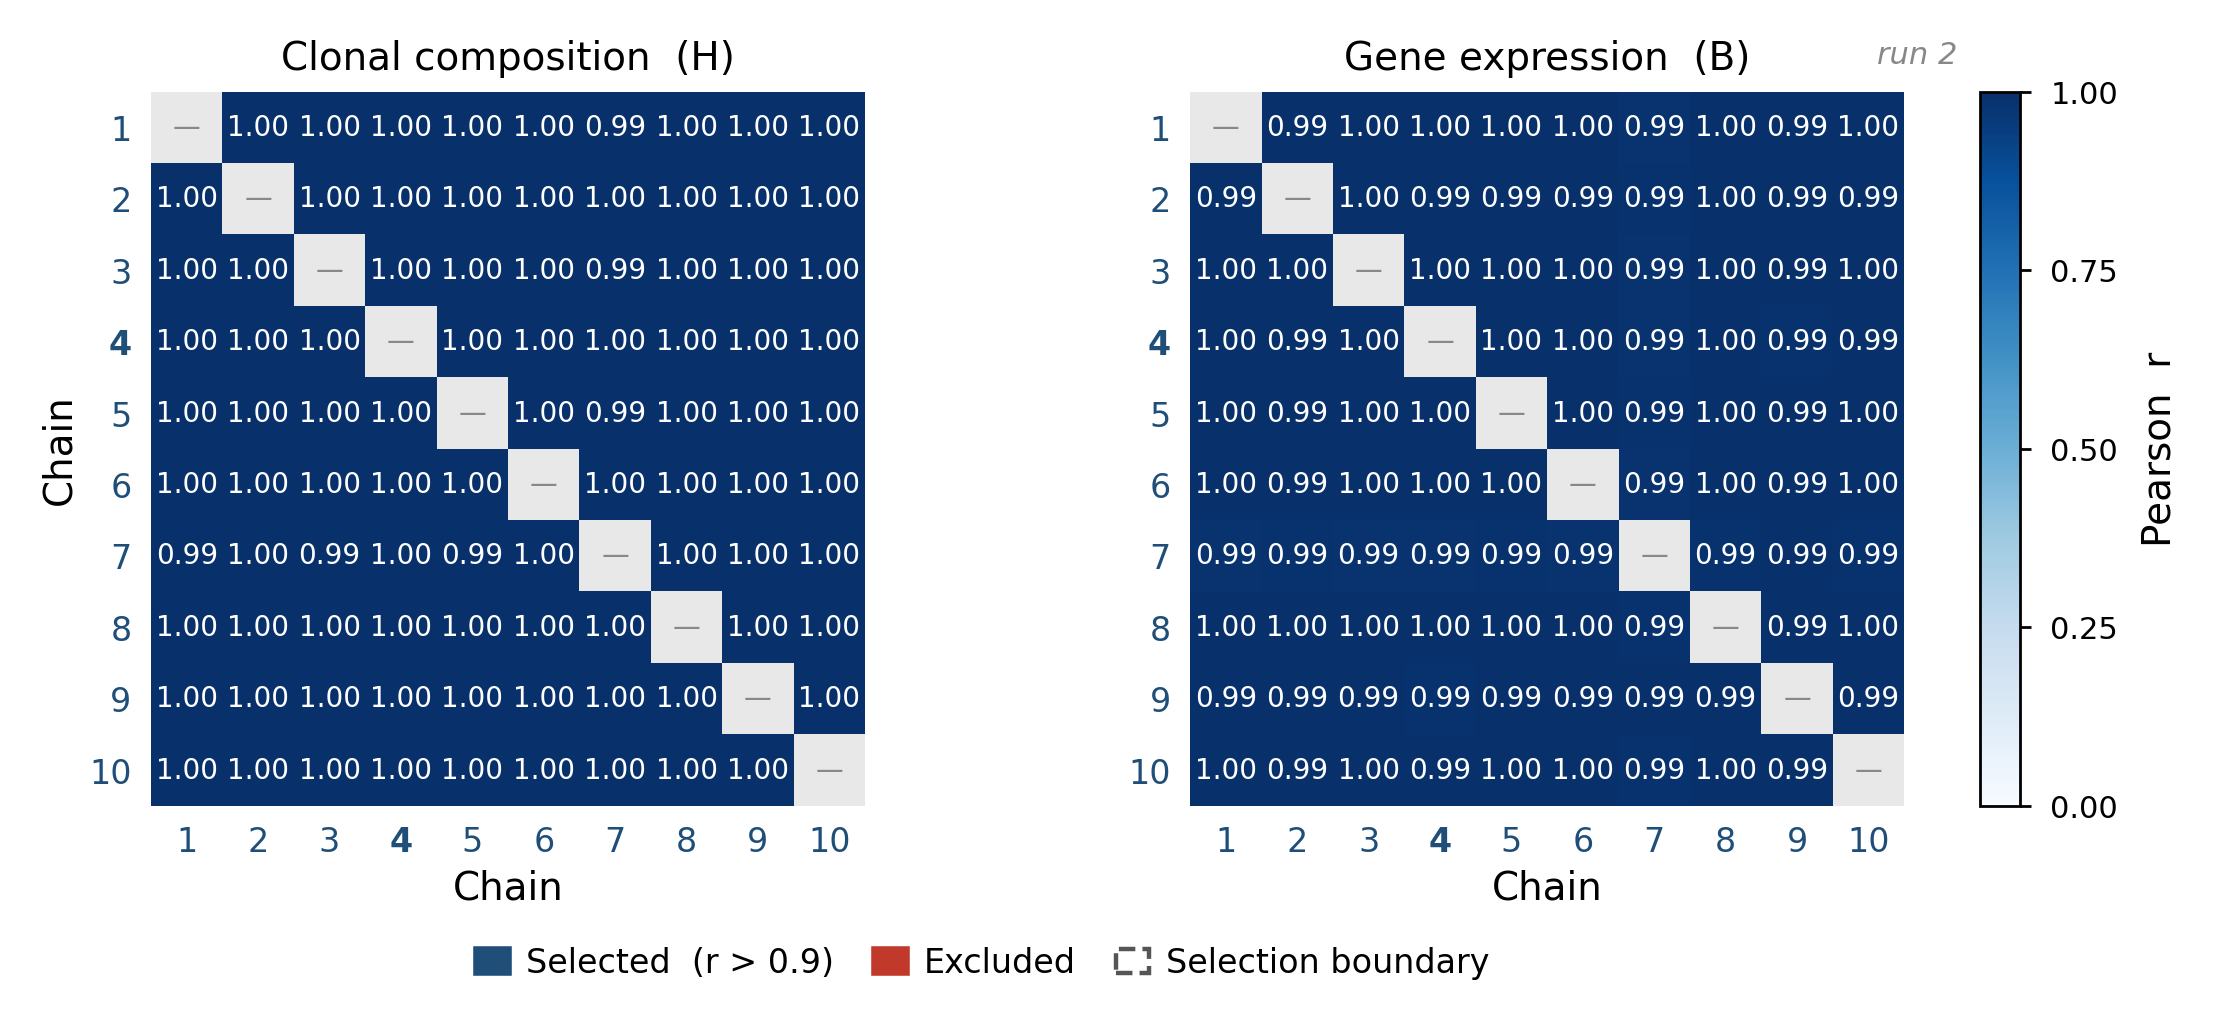
\includegraphics[width=0.78\textwidth]{figures/chain_agreement.png}
  \caption{%
    \textbf{Within-run MCMC chain agreement for the run with the highest
    log-likelihood (run~2).}
    Pairwise Pearson correlation coefficients between the posterior mean
    estimates of all ten independent MCMC chains within the best-performing
    run, shown separately for the clonal composition matrix~$H$
    (spots~$\times$~clones; left) and the clone-specific gene expression
    matrix~$B$ (clones~$\times$~genes; right).
    For each pair of chains $(i,j)$, the Pearson correlation was computed
    between their flattened \texttt{inferred\_H} (resp.\ \texttt{inferred\_B})
    arrays, giving two symmetric $10\times10$ matrices.
    Chain~4 (bold) achieved the highest log-likelihood within the run and
    served as the within-run reference (threshold $r>0.9$); chains are
    reordered so that retained chains (blue labels) appear before the dashed
    selection boundary, with excluded chains (red labels) after it.
    All ten chains were retained (minimum pairwise $r=0.99$ for both $H$
    and $B$), demonstrating that independently initialised Gibbs samplers
    converge to a consistent posterior solution within a single run.%
  }
  \label{fig:chain_agreement}
\end{figure*}

% ── Supplementary Figure S2 ────────────────────────────────────────────────
\begin{figure*}[htbp]
  \centering
  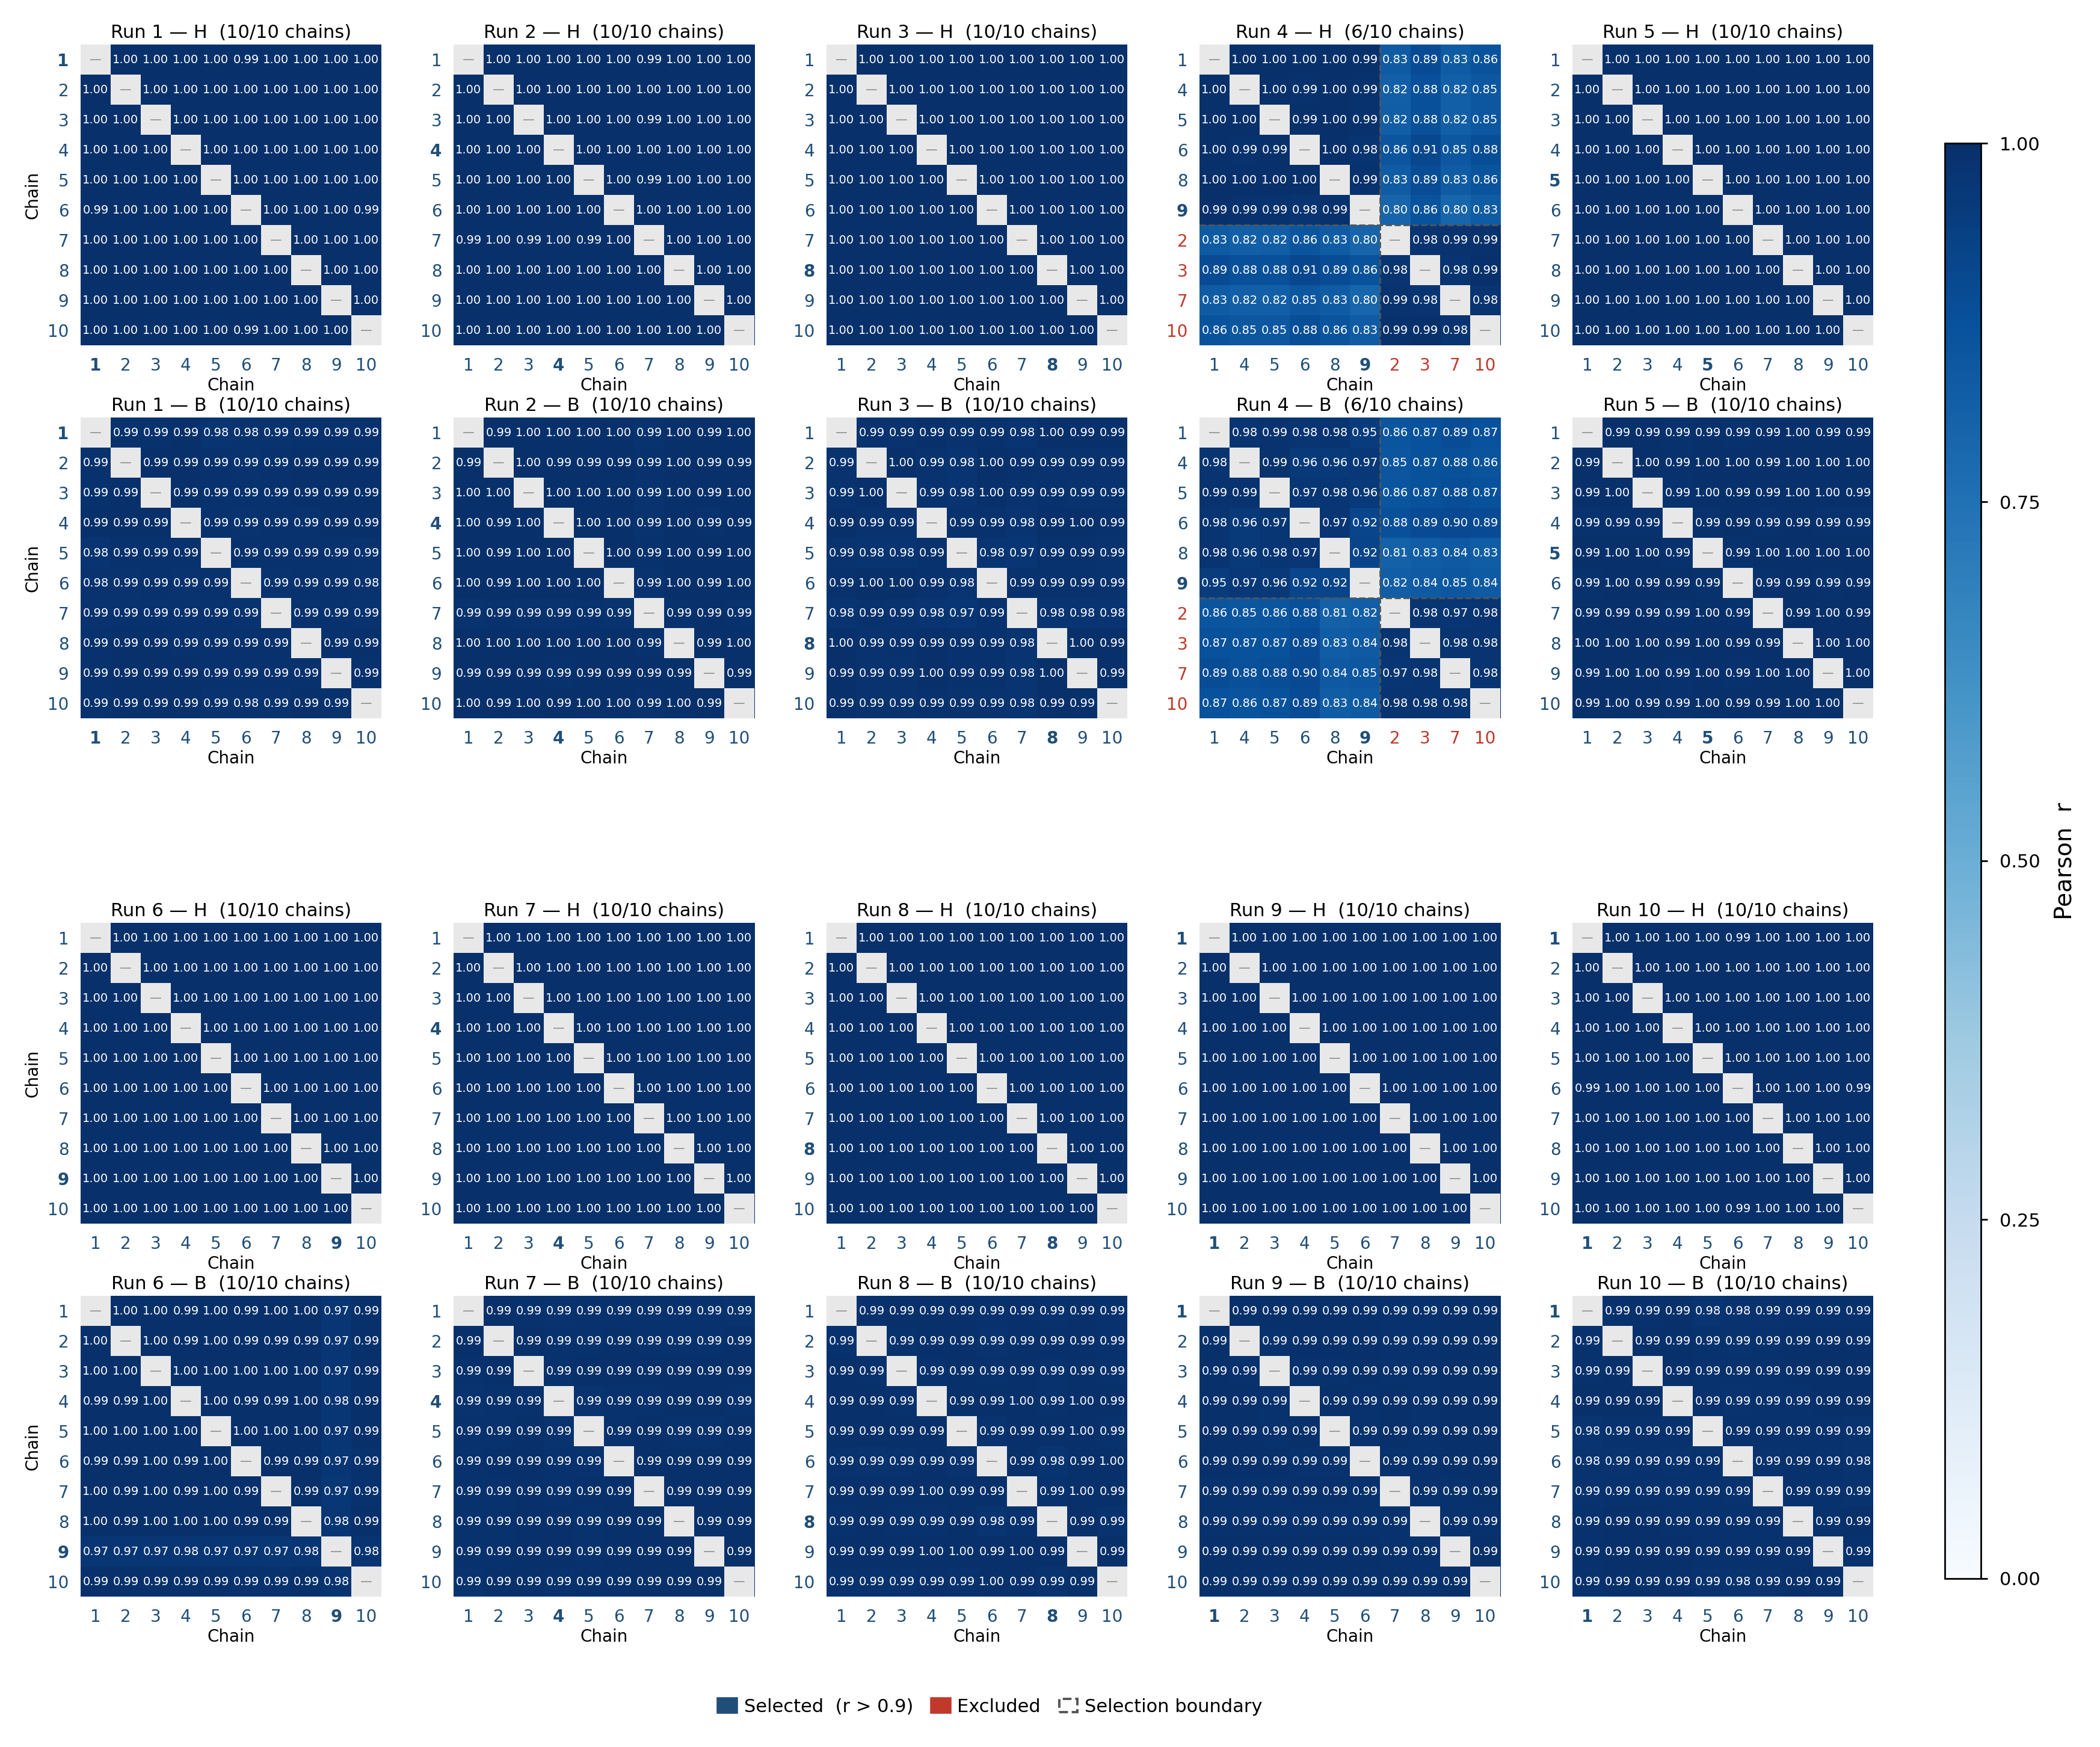
\includegraphics[width=\textwidth]{figures/chain_agreement_supp.png}
  \caption{%
    \textbf{Within-run MCMC chain agreement across all ten independent runs.}
    The same pairwise Pearson correlation procedure as in
    Supplementary Figure~\ref{fig:chain_agreement} was applied independently
    to each of the ten runs.
    Panels are arranged as a $5\times4$ grid: the top two heatmap rows show
    $H$ (clonal composition) and $B$ (gene expression) for runs~1--5;
    the bottom two rows show the same for runs~6--10.
    Within each panel the highest-loglik chain (bold) serves as the
    within-run reference; chains with $r>0.9$ are labelled in blue and
    placed before the dashed selection boundary, while excluded chains are
    labelled in red.  The panel title reports the number of retained chains.
    Nine of ten runs retained all ten chains ($10/10$); run~4 retained
    six ($6/10$), with four chains diverging to a different posterior region.
    In all runs, retained chains show pairwise $r\geq0.97$ for $H$ and
    $r\geq0.87$ for $B$, confirming robust within-run convergence.%
  }
  \label{fig:chain_agreement_supp}
\end{figure*}

% ── Supplementary Figure S3 ────────────────────────────────────────────────
\begin{figure*}[htbp]
  \centering
  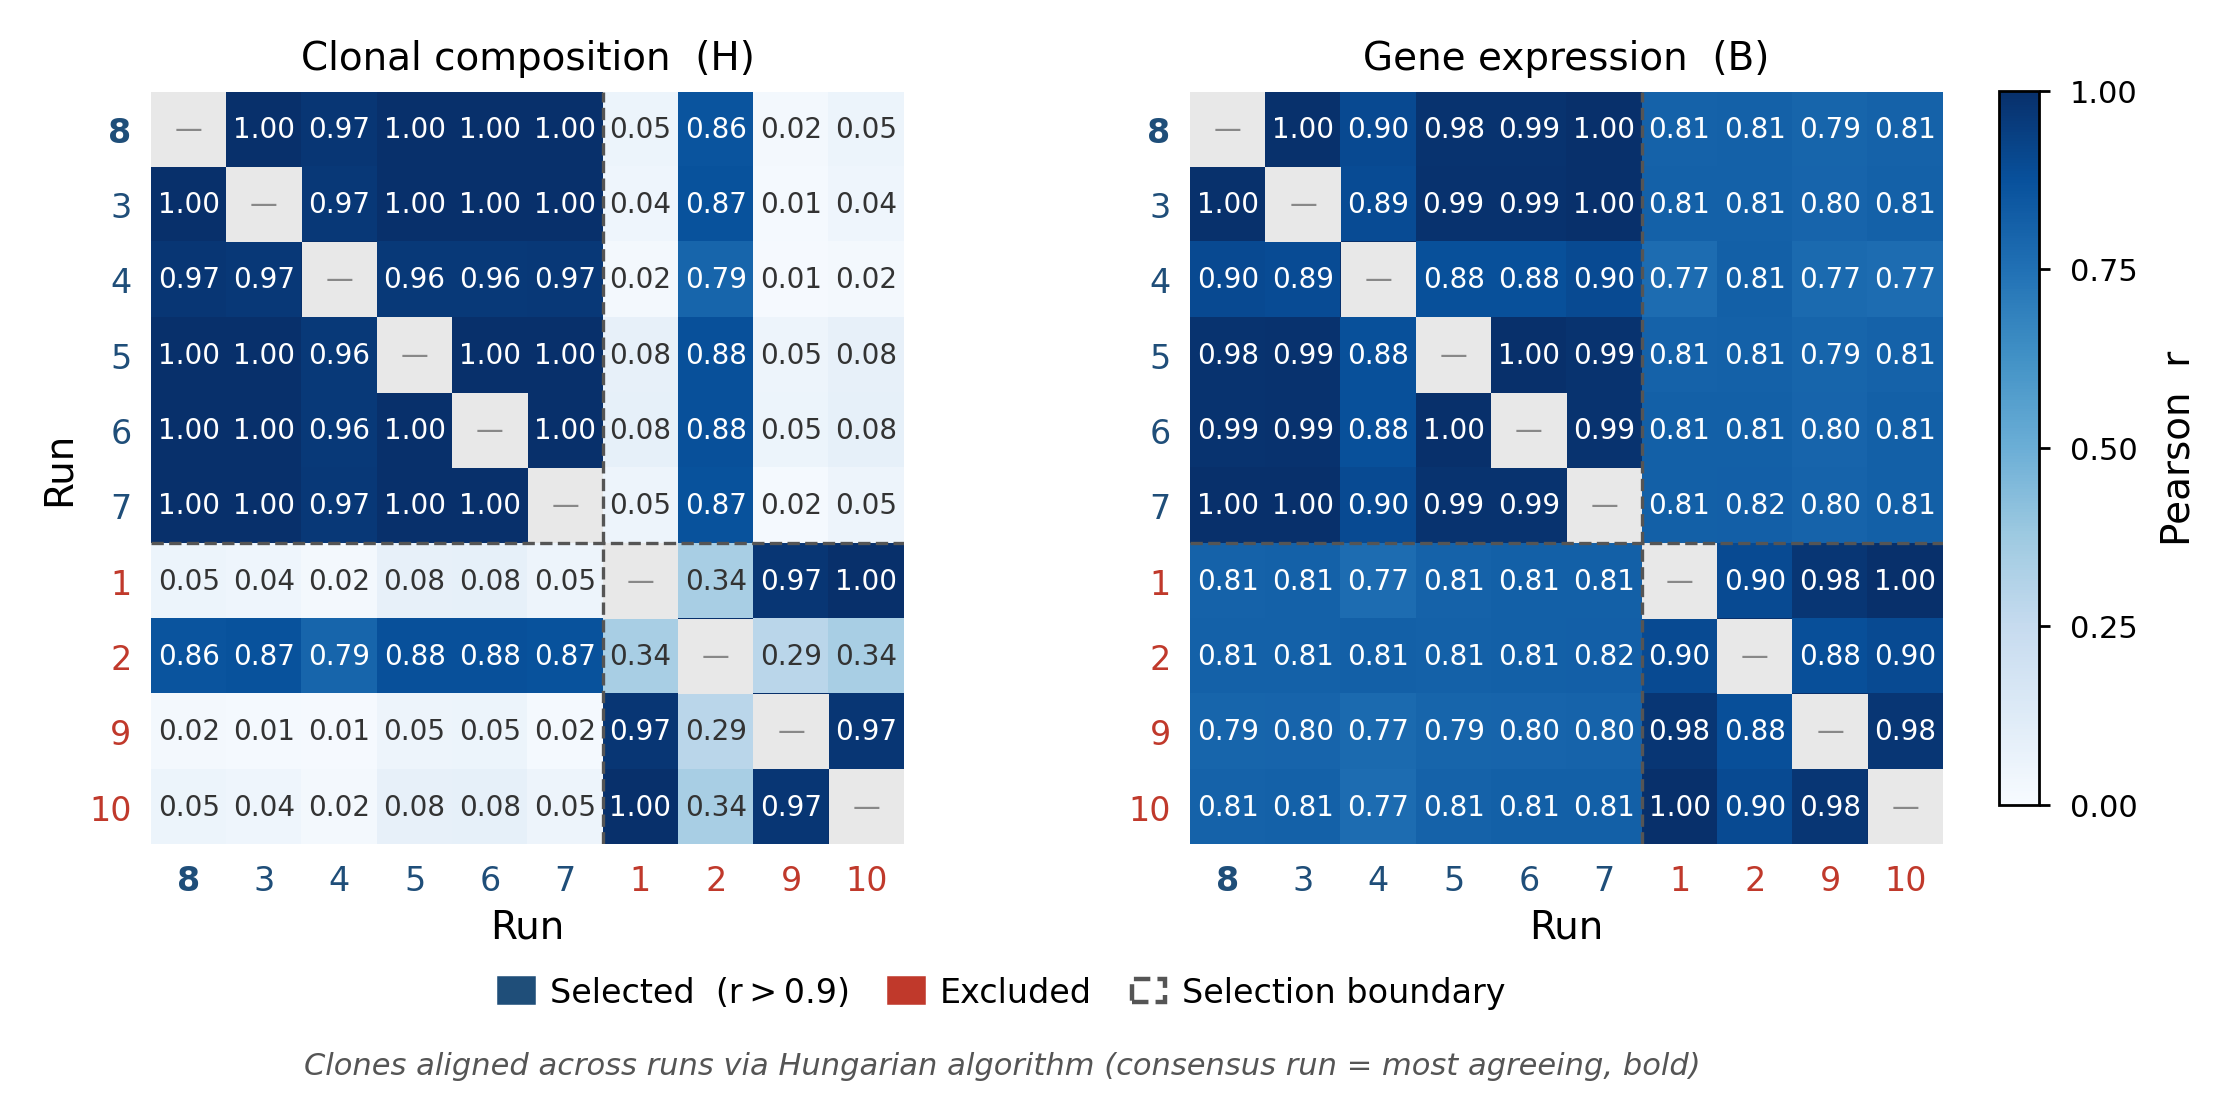
\includegraphics[width=0.78\textwidth]{figures/run_agreement.png}
  \caption{%
    \textbf{Across-run agreement over ten independent runs after
    consensus-based clone alignment.}
    Each run's posterior estimate of $H$ and $B$ was obtained by within-run
    chain selection and averaging (Stage~1).  Clone indices were then aligned
    across runs using the Hungarian algorithm (Stage~2).  Run~8 (bold) was
    identified as the consensus, with six of ten runs satisfying $r>0.9$ on
    the aligned~$H$ (runs~3--8, blue labels); the remaining four runs (red
    labels) were excluded.
    The $10\times10$ pairwise Pearson correlation matrices are shown for the
    aligned~$H$ (left) and~$B$ (right), with runs reordered so the consensus
    group appears first.
    Within the selected group, mean pairwise $r=0.99$ (minimum $0.96$) for
    $H$ and mean $r=0.96$ (minimum $0.88$) for $B$, confirming reproducible
    recovery of clonal composition and gene expression structure.
    The four excluded runs had converged to a different clone ordering that
    could not be reconciled after alignment, consistent with the known
    label-switching behaviour of Bayesian mixture models.%
  }
  \label{fig:run_agreement}
\end{figure*}

% ── Supplementary Figure S4 ────────────────────────────────────────────────
\begin{figure*}[htbp]
  \centering
  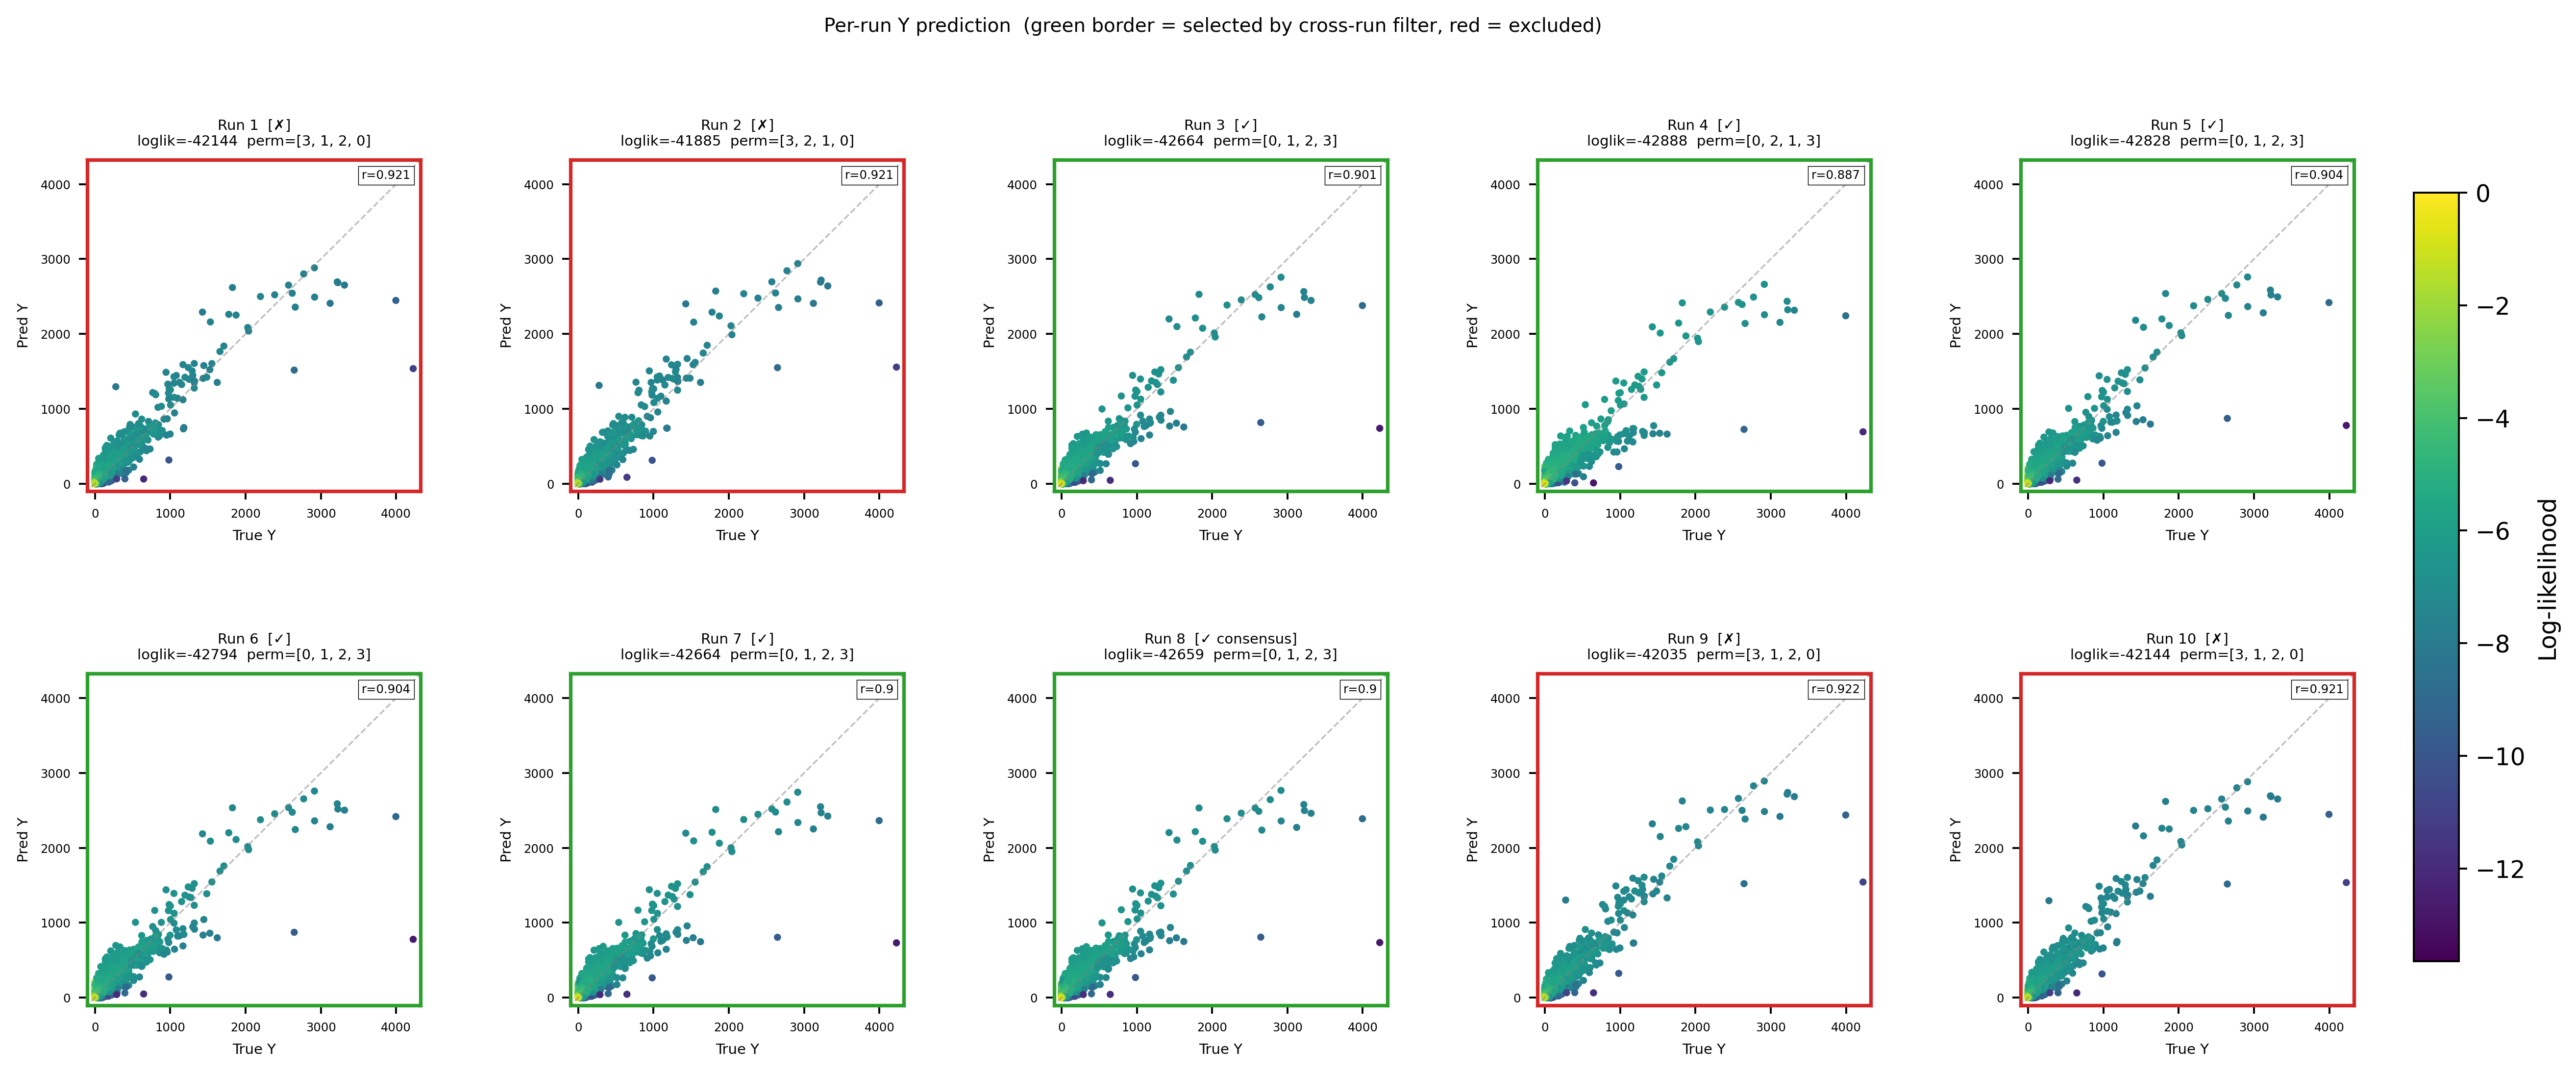
\includegraphics[width=\textwidth]{figures/figure5_supp.png}
  \caption{%
    \textbf{Per-run predicted versus observed gene expression across all ten
    independent runs.}
    For each run, the within-run averaged $H$, $B$, and $N$ were used to
    compute the predicted expression matrix
    $\hat{Y}=\mathrm{diag}(N)\cdot H\cdot B$, with per-section scaling
    applied to account for differing sequencing depths across the three
    tissue sections (P1.2, P2.4, P3.3).
    Each point represents one gene--spot observation, coloured by the
    per-observation negative-binomial log-likelihood.
    The Pearson~$r$ between $Y_{\mathrm{true}}$ and~$\hat{Y}$ is annotated
    in each panel.
    Green borders indicate runs selected by the consensus cross-run filter
    (runs~3--8); red borders indicate excluded runs (runs~1, 2, 9, 10);
    run~8 is additionally labelled as the consensus reference.
    All runs achieve $r\approx0.88$--$0.93$, confirming that every run
    fits the observed expression data well regardless of clone-label
    orientation, and that exclusion of runs~1, 2, 9, and~10 is driven by
    label switching rather than inferior predictive accuracy.%
  }
  \label{fig:figure5_supp}
\end{figure*}

\subsection*{Runtime analysis}
\rev{We measured wall-clock runtimes across all simulation replicates and all
real-data runs to characterise the computational demands of ClonalGE relative
to its predecessor Tumoroscope.
All experiments were executed on the same hardware (single workstation, CPU
only), so runtimes are directly comparable across methods.}

\paragraph{Simulated data.}
For each of the three simulation setups (\textit{basic}, \textit{low
expression variance}, \textit{high coverage}) we timed 20 independent
replicates for each of the three methods: Tumoroscope, ClonalGE with a single
MCMC chain (ClonalGE 1-chain), and ClonalGE with five parallel MCMC chains
with best-chain selection (ClonalGE 5-chains).
All methods used the same iteration bounds (minimum 10\,000, maximum 30\,000
iterations, saved every 5th sample) and stopped early upon satisfying the
99.5\% Geweke convergence criterion.
Summary statistics (mean $\pm$ standard deviation and range) are given in
Table~\ref{tab:runtime}; runtime distributions are shown in
Supplementary Figure~\ref{fig:runtime}.

\begin{figure*}[htbp]
  \centering
  \rev{
\includegraphics[width=0.85\textwidth]{figures/figure_runtime.png}}
  \caption{%
    \textbf{Supplementary Figure~\ref{fig:runtime}: Runtime distributions for ClonalGE and Tumoroscope.}
    \rev{Wall-clock runtimes (minutes) across 20 independent replicates for each
    simulation configuration and method.
    Box plots show median, interquartile range, and 1.5$\times$IQR whiskers;
    individual replicates are overlaid as points.
    Dashed vertical lines mark the median runtime of Tumoroscope for reference.
    Outliers in ClonalGE conditions correspond to replicates that ran to the
    maximum iteration bound (30\,000) before the Geweke convergence criterion
    was satisfied.}
  }
  \label{fig:runtime}
\end{figure*}


\paragraph{Real prostate cancer data.}
We ran ClonalGE on the prostate cancer dataset (294 spots, $K=4$ clones,
$I$ mutations, $G=1000$ genes) 20 times with different random seeds, each
time executing 10 parallel MCMC chains.
The mean wall-clock time per run was $769.8 \pm 187.7$\,min
(median 784.4\,min, range 520.3--1047.4\,min).


\begin{table}[ht]
\centering
\rev{
\caption{%
\textbf{Wall-clock runtime of ClonalGE and Tumoroscope across all simulation
conditions and on real prostate cancer data.}
Values are mean\,$\pm$\,SD (range in parentheses) in minutes, computed over
20 independent replicates for each simulation setup and method, and over 20
independent runs for the real prostate data.
All simulated experiments used the same iteration bounds (minimum 10\,000,
maximum 30\,000 iterations) and the same 99.5\% Geweke convergence stopping
criterion.
The elevated mean and standard deviation for Tumoroscope in the
\textit{basic} and \textit{low expression variance} conditions reflect
slower and more variable convergence in the absence of gene expression
information.
For ClonalGE 5-chains, five MCMC chains were executed in parallel on
separate CPU cores; total wall-clock time therefore scales sub-linearly with
the number of chains.
Runtimes exceeding $\approx$60\,min in the ClonalGE conditions (visible in
the elevated maxima) correspond to runs that required the full 30\,000
iterations before the convergence criterion was met.
The \textit{high coverage} setup converges faster for all methods because
higher read depth produces sharper likelihood gradients.
For the real prostate cancer data (294 spots, $K=4$ clones, $G=1000$ genes),
each run comprised 10 parallel MCMC chains; the substantially longer runtimes
relative to simulated data reflect the ten-fold larger number of genes
and the higher chain count.
}
\label{tab:runtime}
\small
\begin{tabular}{lccc}
\hline
\textbf{Method}
  & \textbf{\textit{Basic}}
  & \textbf{\textit{Low expression variance}}
  & \textbf{\textit{High coverage}} \\
\hline
Tumoroscope
  & $37.1 \pm 10.2$ (16.9--46.2)
  & $41.5 \pm 9.7$ (16.8--47.1)
  & $19.1 \pm 0.2$ (18.7--19.6) \\
ClonalGE (1 chain)
  & $21.9 \pm 0.1$ (21.7--22.1)
  & $23.7 \pm 8.2$ (21.6--59.3)
  & $23.7 \pm 0.1$ (23.3--24.0) \\
ClonalGE (5 chains)
  & $28.4 \pm 13.3$ (22.7--60.3)
  & $22.8 \pm 0.2$ (22.6--23.2)
  & $24.9 \pm 0.2$ (24.5--25.3) \\
\hline
\multicolumn{4}{l}{%
\textit{Real data (prostate cancer, 10 chains per run):}
$769.8 \pm 187.7$\,min (520.3--1047.4\,min), $n=20$ runs.} \\
\hline
\end{tabular}
}
\end{table}

% Supplementary Table S1: ClonalGE model variables and parameters
% Paste this into the supplementary section of oup-authoring-template.tex
% Requires: \usepackage{booktabs}, \usepackage{array}, \usepackage{makecell}
% (booktabs and array are standard in OUP template; add makecell to preamble if needed)

% Supplementary Table S1: ClonalGE model variables and parameters
% Paste this into the supplementary section of oup-authoring-template.tex
% Requires: \usepackage{array}  (standard in OUP template)

\begin{table*}[!ht]
\caption{%
  \textbf{Supplementary Table S1.}
  Complete list of all variables and parameters in the ClonalGE model.
  Index ranges: $k \in \{1,\ldots,K\}$ (clones), $s \in \{1,\ldots,S\}$ (spots),
  $g \in \{1,\ldots,G\}$ (genes), $i \in \{1,\ldots,I\}$ (mutation loci),
  $j \in \{1,\ldots,J\}$ (tissue sections).
}\label{tab:variables}
\renewcommand{\arraystretch}{1.35}
% Column widths: symbol(1cm) | name(3.2cm) | dimension(1.8cm) | status(2.2cm) | description(fills rest)
\begin{tabular}{@{} p{1cm} p{3.2cm} p{1.8cm} p{2.2cm} p{6.5cm} @{}}
\hline
\textbf{Symbol} & \textbf{Name} & \textbf{Dimension} & \textbf{Obs./Latent} & \textbf{Description} \\
\hline
\multicolumn{5}{@{}l}{\textit{Indices and dimensions}} \\
\hline
$K$ & Number of clones        & scalar & input & Number of clones inferred from DNA-seq \\
$S$ & Number of spots         & scalar & input & Number of cancerous ST spots \\
$G$ & Number of genes         & scalar & input & Number of genes analysed in ST data \\
$I$ & Number of mutations     & scalar & input & Number of somatic SNV loci shared between DNA-seq and ST \\
$J$ & Number of sections      & scalar & input & Number of tissue sections \\
\hline
\multicolumn{5}{@{}l}{\textit{Observed variables (given as input to the model)}} \\
\hline
$F_k$       & Clone frequency        & $K$     & observed & Frequency of clone $k$ in the whole sample, estimated from DNA-seq \\
$C_{ik}$    & Clone genotype matrix  & $I \times K$ & observed & Fraction of alleles of clone $k$ carrying a mutation at locus $i$; values in $[0,1]$ \\
$D_{is}$    & Total read depth       & $I \times S$ & observed & Total read count at mutation locus $i$ in spot $s$ from ST data \\
$A_{is}$    & Alternated read count  & $I \times S$ & observed & Mutated (alternated) read count at locus $i$ in spot $s$ from ST data \\
$Y_{sg}$    & Spot gene expression   & $S \times G$ & observed & UMI count of gene $g$ in spot $s$ from ST data \\
$\Lambda_s$ & Expected cell count    & $S$     & observed & Cell count at spot $s$ estimated from H\&E images; used as Poisson rate for $N_s$ \\
\hline
\multicolumn{5}{@{}l}{\textit{Latent variables (inferred by Gibbs/MH sampling)}} \\
\hline
$\Pi_{sk}$  & Clone presence prior   & $S \times K$ & latent & Beta-distributed probability that clone $k$ is present in spot $s$ \\
$Z_{sk}$    & Clone presence indicator & $S \times K$ & latent & Binary; $Z_{sk}=1$ if clone $k$ is present in spot $s$ \\
$G_{sk}$    & Unnorm.\ clone abundance & $S \times K$ & latent & Gamma-distributed unnormalised abundance of clone $k$ in spot $s$ \\
$H_{sk}$    & Clone fraction         & $S \times K$ & latent & Fraction of spot $s$ occupied by clone $k$; $H_{sk} = G_{sk}/\sum_l G_{sl}$ \\
$\Phi_{ik}$ & Per-cell read rate     & $I \times K$ & latent & Average read count at locus $i$ per cell of clone $k$ \\
$N_s$       & Cell count             & $S$     & latent & Number of cells in spot $s$; Poisson-distributed with rate $\Lambda_s$ \\
$B_{kg}$    & Clonal gene expression & $K \times G$ & latent & Average expression of gene $g$ per cell in clone $k$; Gamma-distributed \\
\hline
\multicolumn{5}{@{}l}{\textit{Fixed hyperparameters and pre-estimated parameters}} \\
\hline
$\zeta_s$   & Clone-count hyperparam. & $S$  & hyperparameter & Controls expected number of clones per spot; shapes Beta prior on $\Pi_{sk}$ \\
$F_0$       & Absent-clone pseudo-count & scalar & hyperparameter & Gamma shape for $G_{sk}$ when $Z_{sk}=0$; set to a small positive value \\
$r$         & $\Phi$ shape hyperparam. & scalar & hyperparameter & Shape parameter of Gamma prior on $\Phi_{ik}$; estimated from data \\
$q$         & $\Phi$ rate hyperparam.  & scalar & hyperparameter & Rate parameter of Gamma prior on $\Phi_{ik}$; estimated from data \\
$\alpha_g$  & $B$ shape hyperparam.    & $G$   & hyperparameter & Per-gene shape parameter of Gamma prior on $B_{kg}$; estimated from data \\
$\beta$     & $B$ rate hyperparam.     & scalar & hyperparameter & Rate parameter of Gamma prior on $B_{kg}$; estimated from data \\
$p_g$       & NB success probability   & $G$   & hyperparameter & Success probability of Negative Binomial distribution for $Y_{sg}$; estimated from data \\
$t_j$       & Section scaling factor   & $J$   & hyperparameter & Multiplicative scaling factor correcting for batch effects across section $j$ \\
$\omega_B$  & $B$ variance correction  & scalar & hyperparameter & Correction constant for underestimation of $\beta$; fixed to $2$ \\
$\omega_\phi$ & $\Phi$ variance correction & scalar & hyperparameter & Correction constant for underestimation of $r$; fixed to $2$ \\
\hline
\end{tabular}
\end{table*}

% ── Supplementary Figure: Hyperparameter sensitivity ───────────────────────
\begin{figure*}[htbp]
  \centering
  \rev{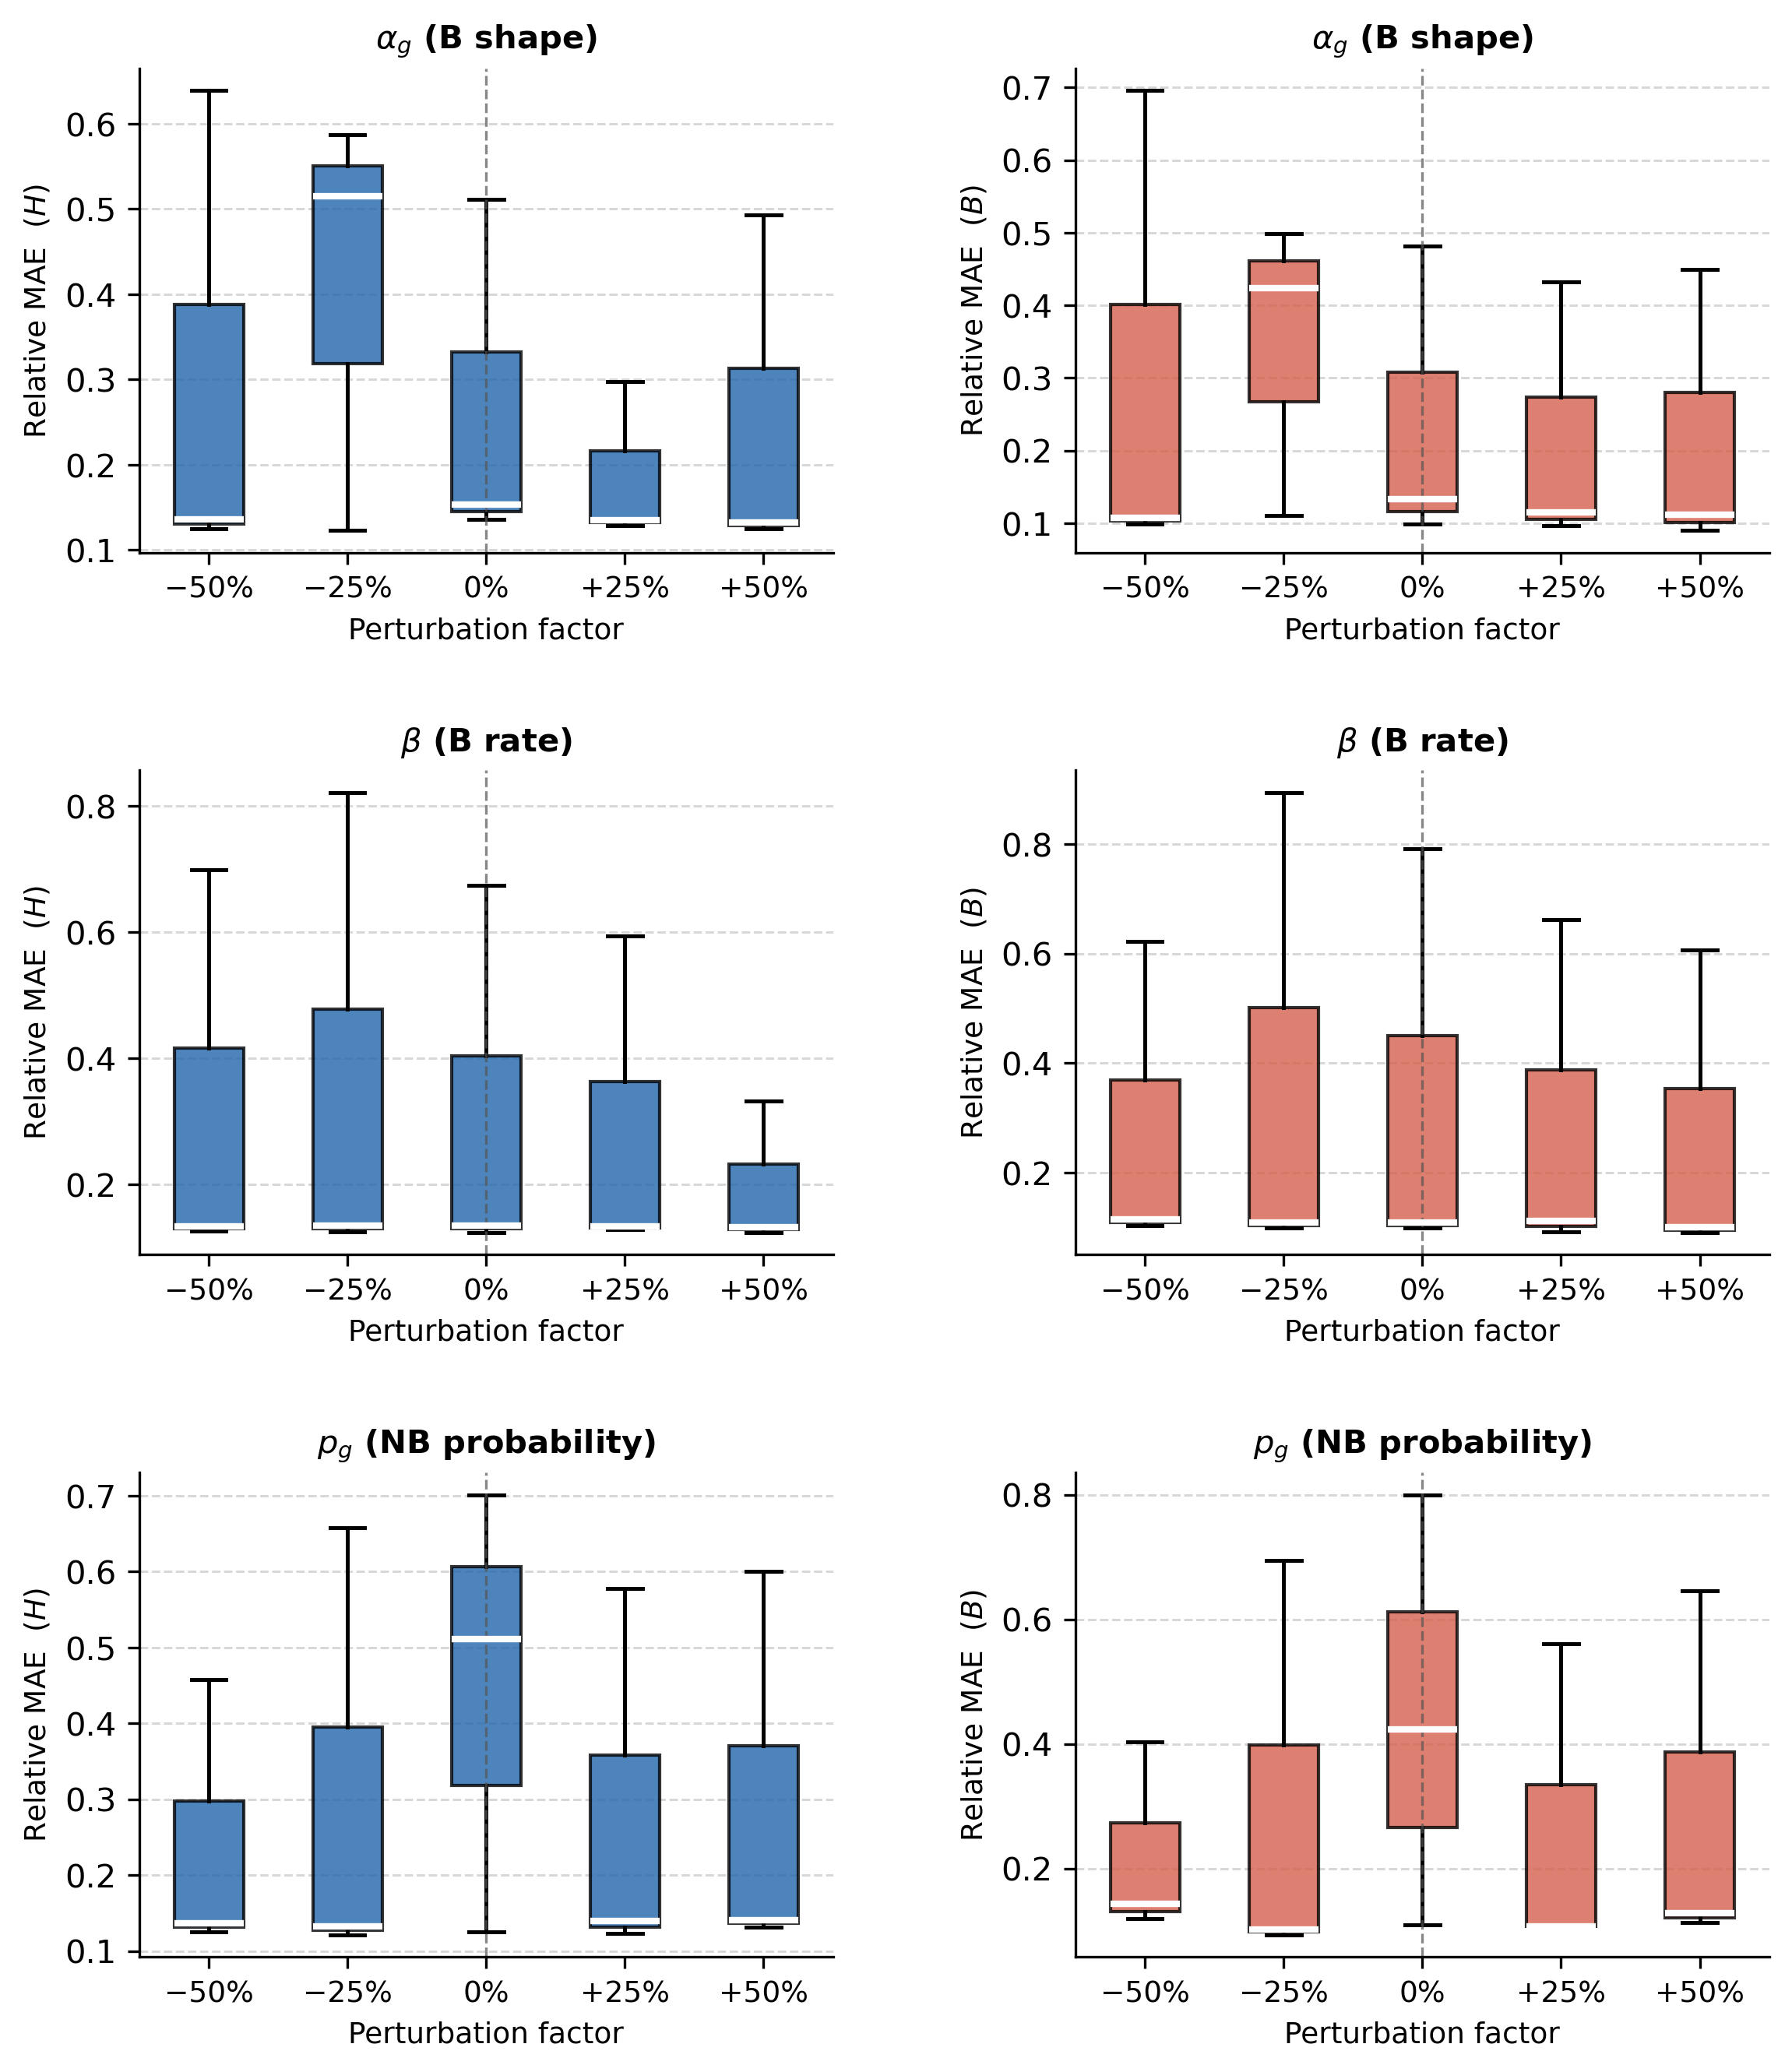
\includegraphics[width=0.85\textwidth]{figures/sensitivity_analysis.png}}
  \caption{%
    \textbf{Supplementary Figure: Hyperparameter sensitivity of ClonalGE.}
    \rev{Relative MAE for clone-fraction recovery ($H$, left) and clonal gene
    expression recovery ($B$, right) as a function of hyperparameter perturbation
    factor applied to $\alpha_g$ (Gamma shape of the $B$ prior; top row),
    $\beta$ (Gamma rate of the $B$ prior; middle row), and $p_g$
    (Negative Binomial success probability; bottom row).
    Each boxplot summarises 3 independent simulation replicates of the
    \textit{normal} configuration; the factor 1.0 (dashed line) corresponds to
    the true (data-derived) hyperparameter value.}
  }
  \label{fig:sensitivity}
\end{figure*}

% ── Supplementary Figure: GSEA ─────────────────────────────────────────────
\begin{figure*}[htbp]
  \centering
  \rev{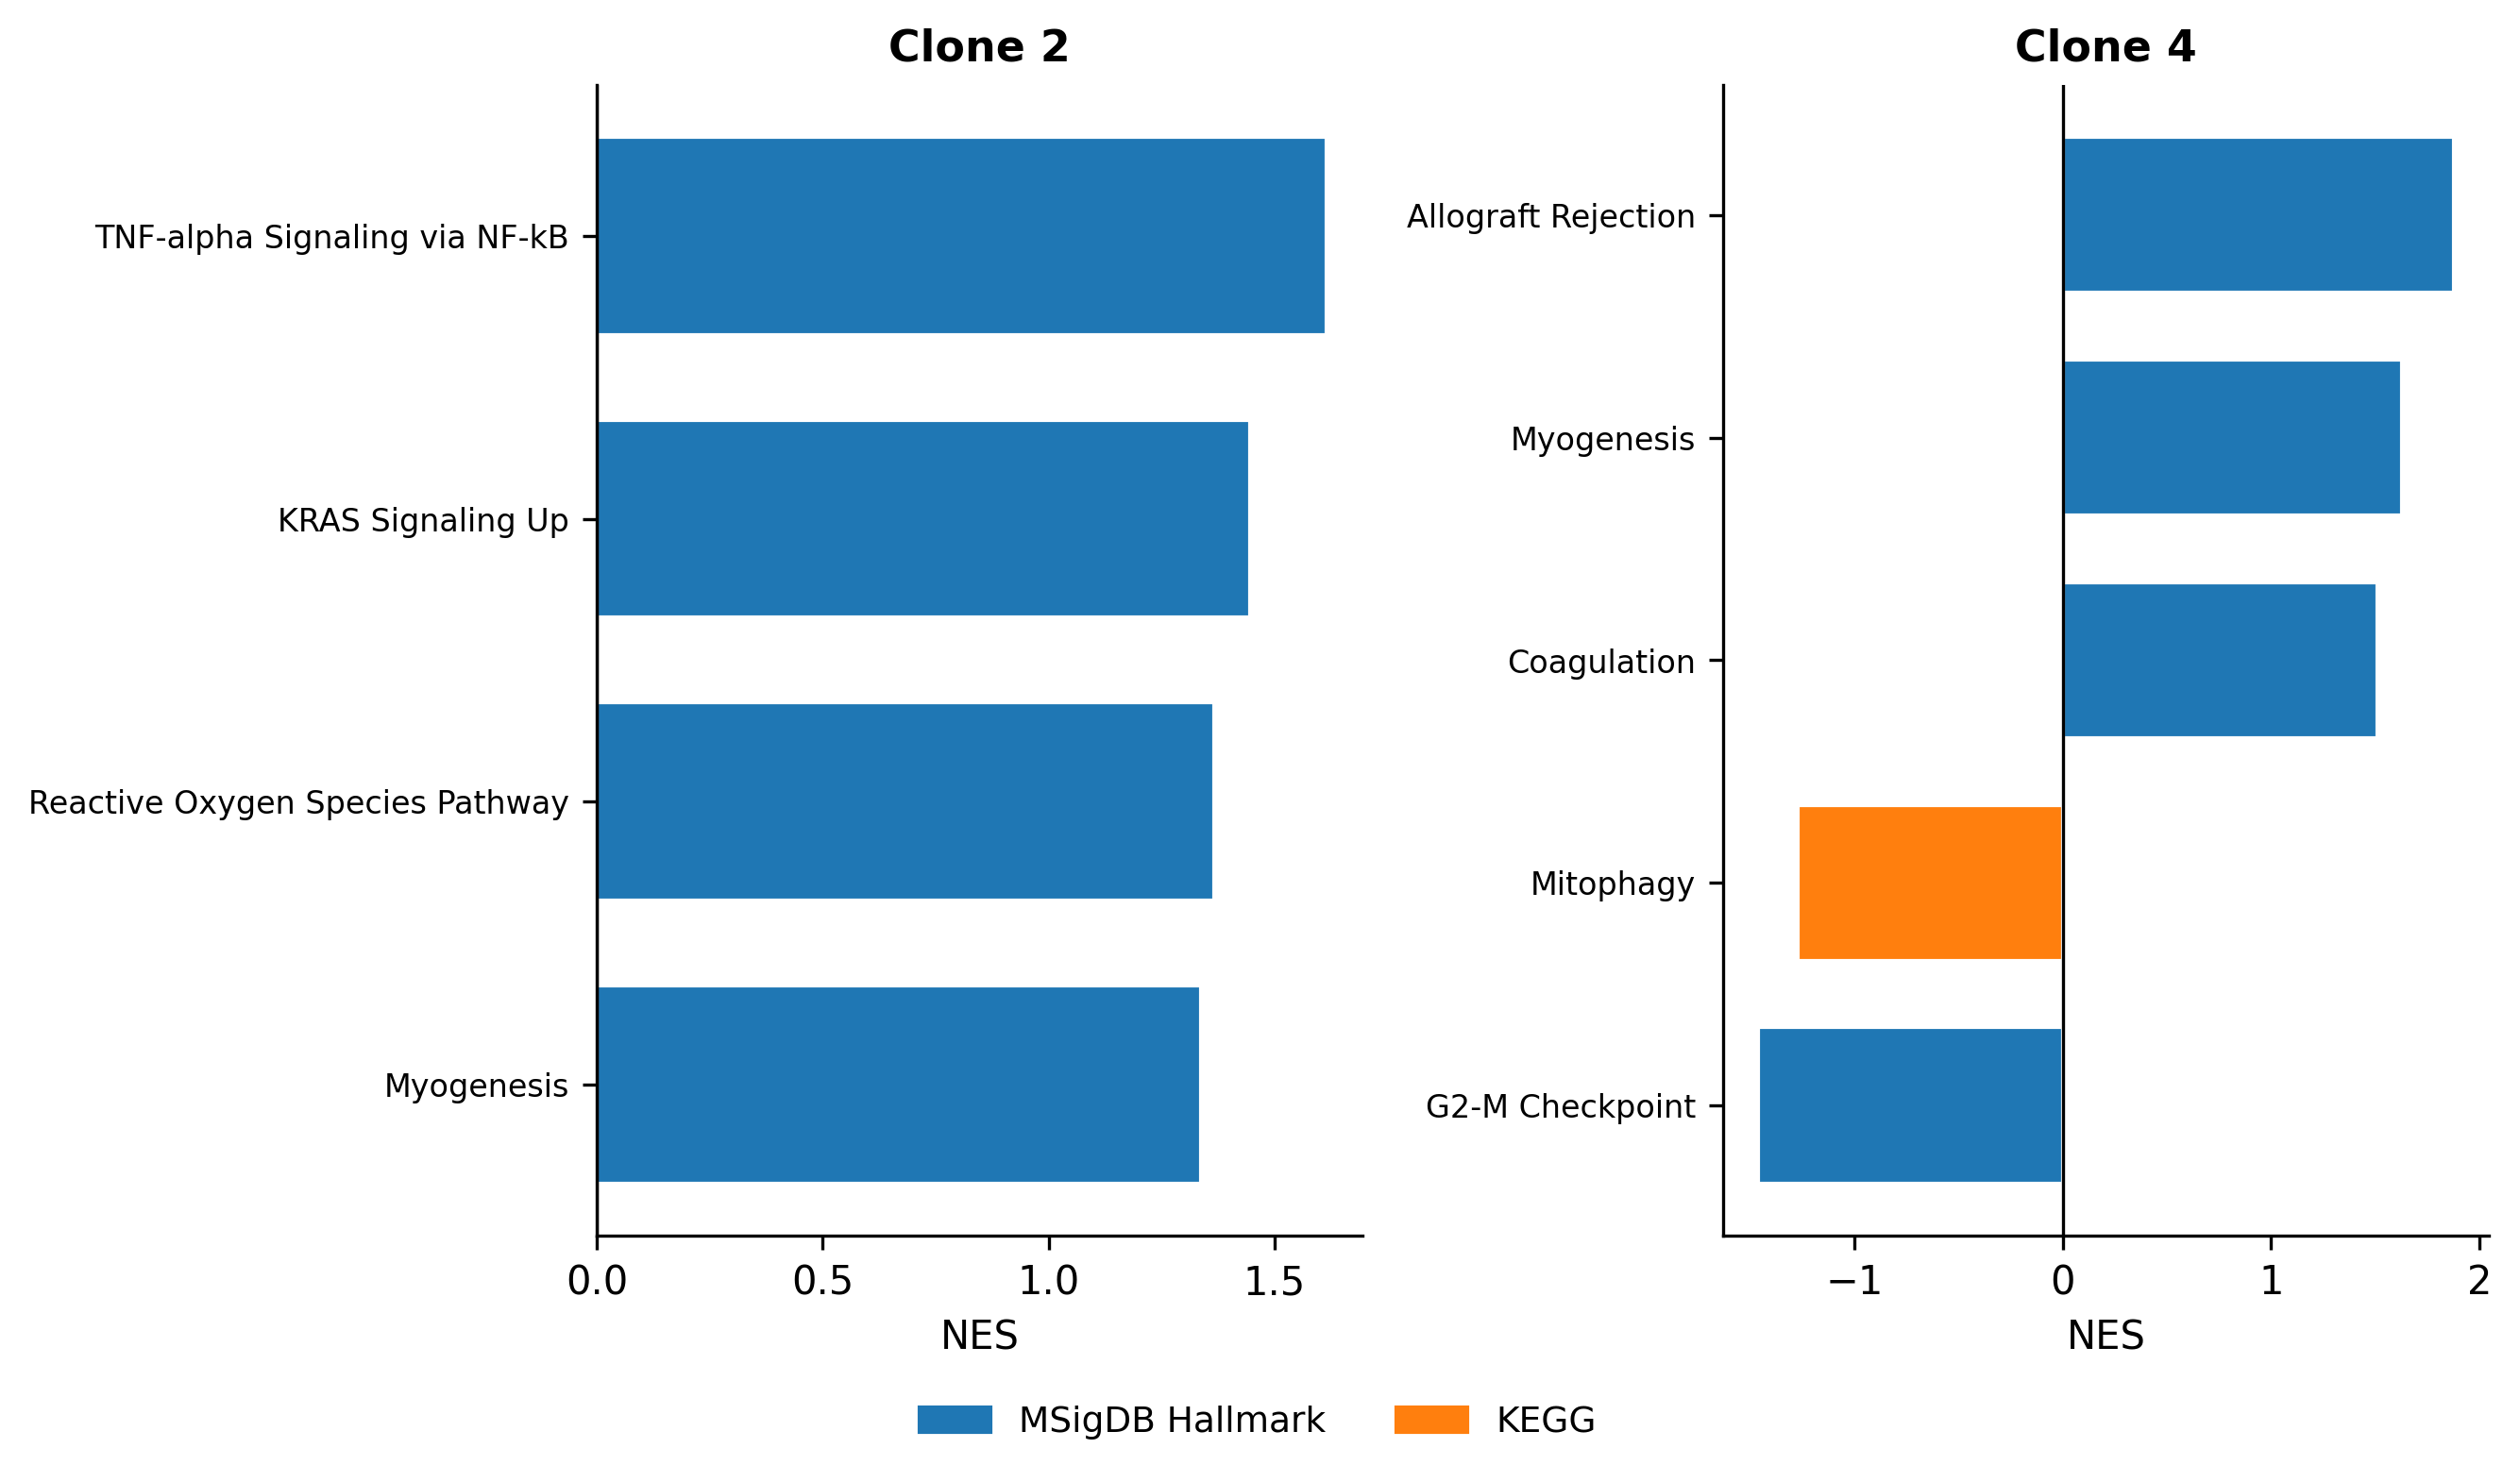
\includegraphics[width=0.90\textwidth]{figures/gsea_results.png}}
  \caption{%
    \textbf{Supplementary Figure: Gene Set Enrichment Analysis (GSEA) for clone-specific gene expression.}
    \rev{Pre-ranked GSEA results for each of the $K$ inferred clones (panels)
    using MSigDB Hallmark gene sets.
    Genes were ranked by the posterior probability
    $P(B_{k,g} > \bar{B}_{\text{other},g} \mid \text{Data})$ that clone $k$
    overexpresses gene $g$ relative to all other clones.
    Normalised enrichment scores (NES) are shown for gene sets with
    false-discovery-rate-adjusted $q < 0.25$.
    Positive NES indicates enrichment among clone-specific over-expressed genes.}
  }
  \label{fig:gsea}
\end{figure*}

% ── Supplementary Figure: Assumption-violating simulations ─────────────────
\begin{figure*}[htbp]
  \centering
  \rev{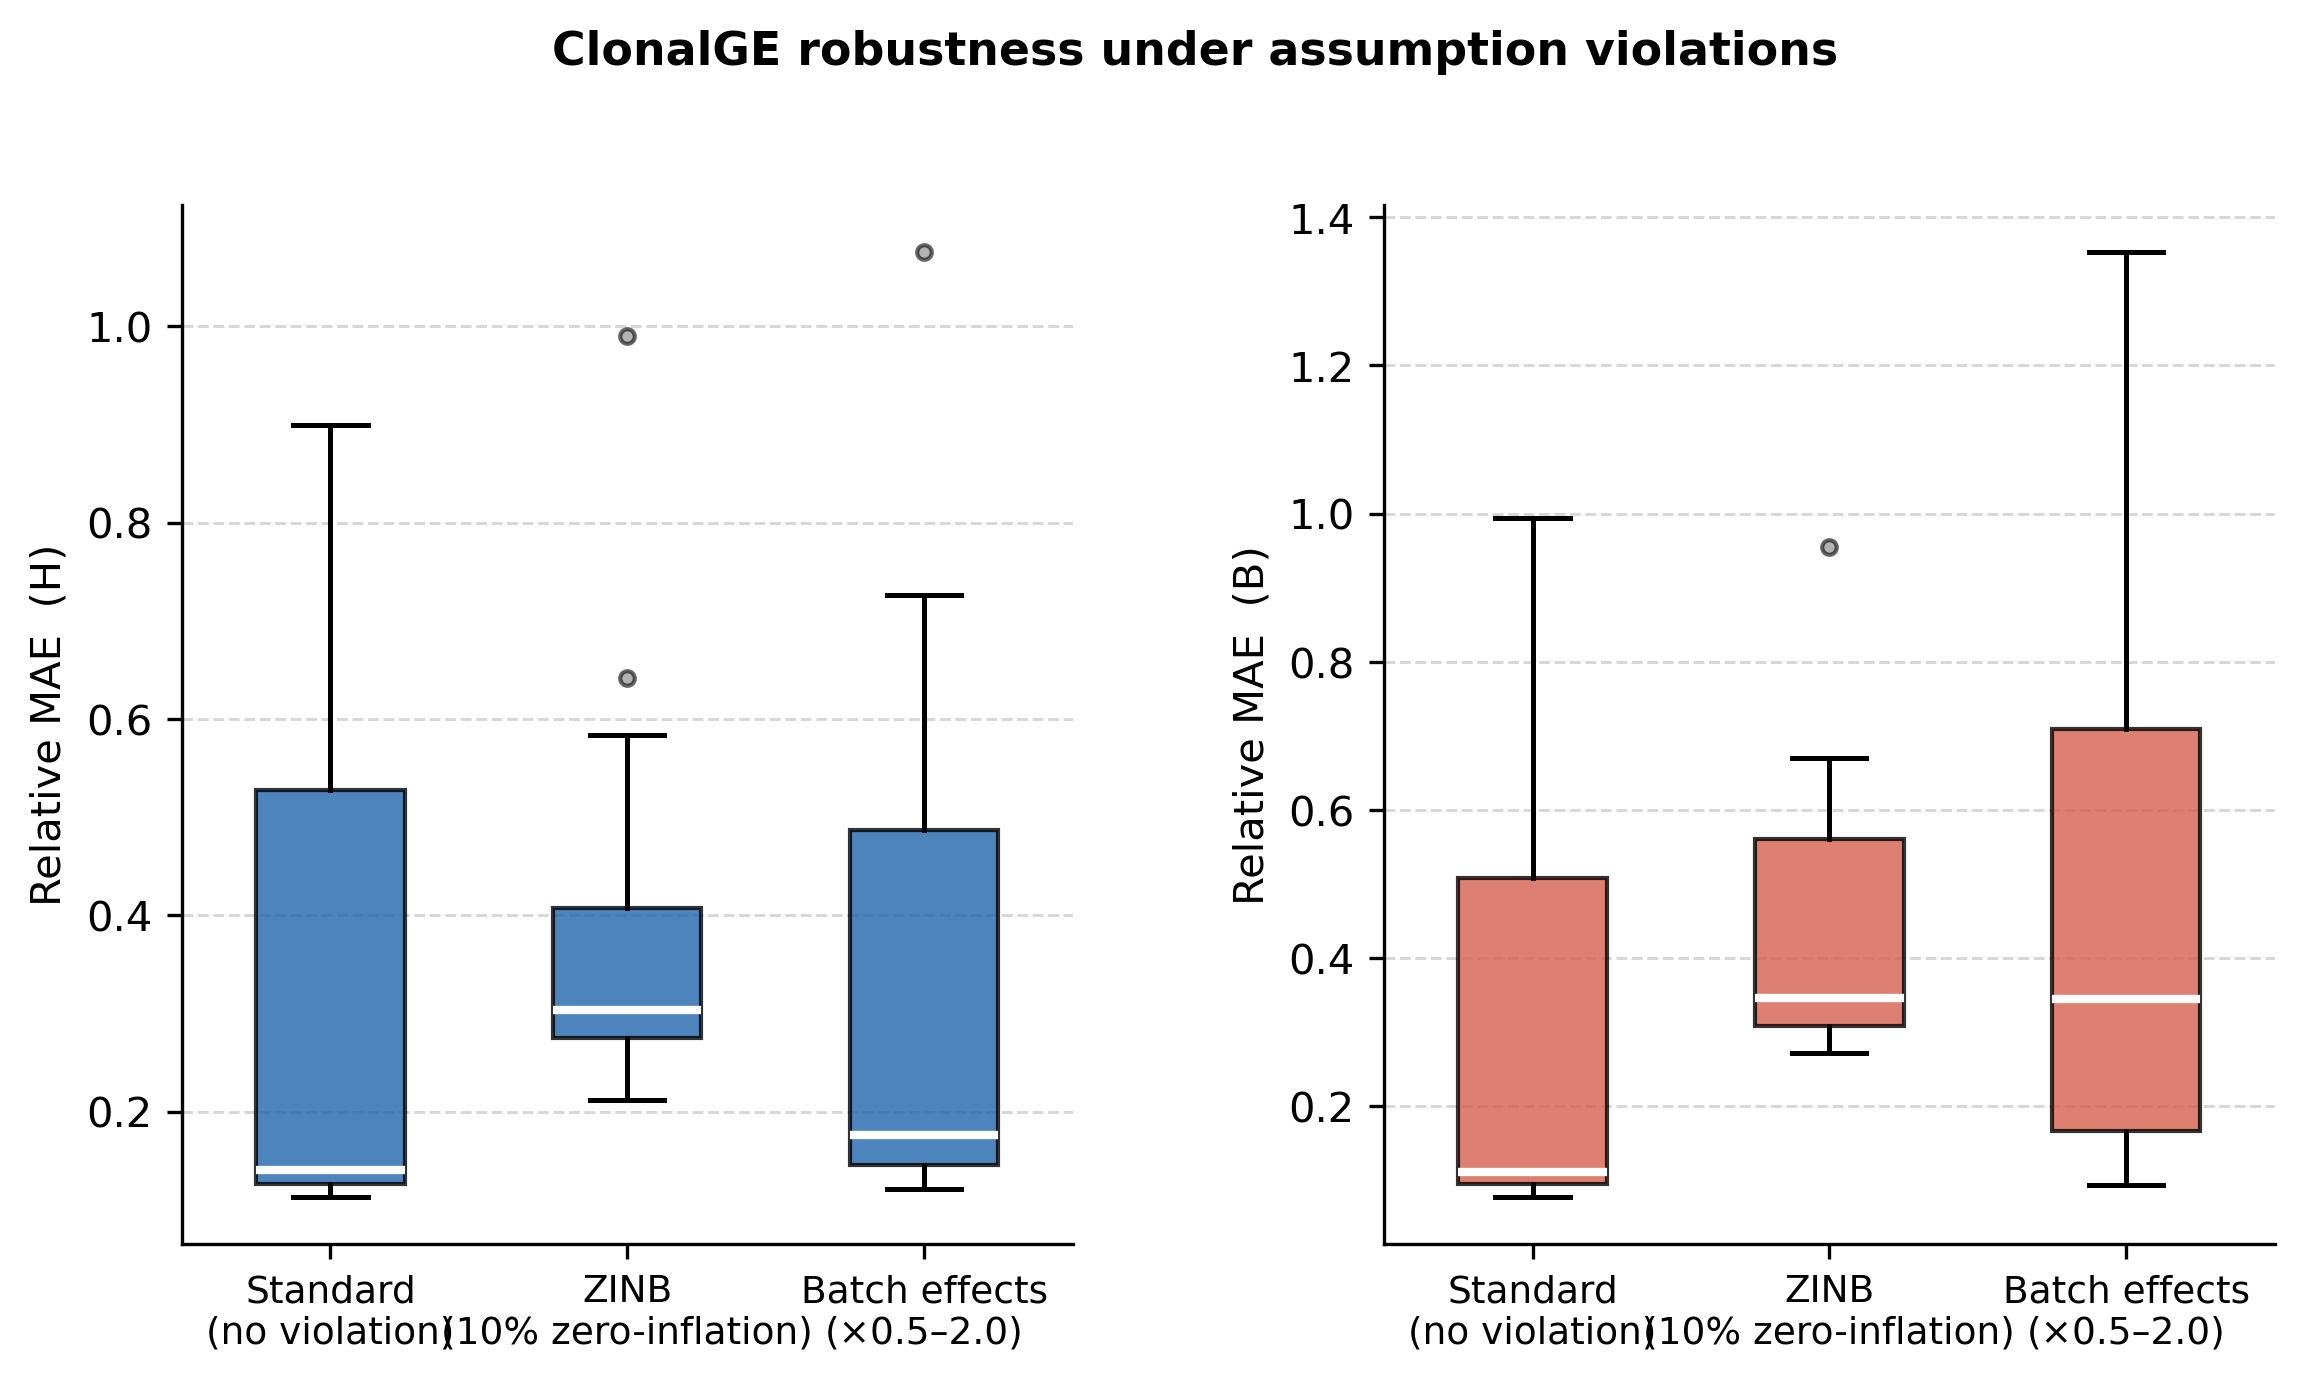
\includegraphics[width=0.85\textwidth]{figures/violated_simulations.png}}
  \caption{%
    \textbf{Supplementary Figure: ClonalGE performance under assumption-violating simulation conditions.}
    \rev{Relative MAE for $H$ and $B$ under three conditions: (i) standard simulation
    (ground truth, no assumption violations), (ii) zero-inflated Negative Binomial
    gene expression (10\% zero-inflation rate), and (iii) section-level batch effects
    (multiplicative factors drawn from $\text{Uniform}(0.5, 2.0)$).
    Each boxplot shows 20 independent replicates; lower values indicate better
    inference accuracy.
    Results demonstrate that ClonalGE remains robust to moderate deviations from
    the NB distributional assumption and to batch effects of this magnitude.}
  }
  \label{fig:violated}
\end{figure*}

\end{document}
